\documentclass[]{book}
\usepackage{lmodern}
\usepackage{amssymb,amsmath}
\usepackage{ifxetex,ifluatex}
\usepackage{fixltx2e} % provides \textsubscript
\ifnum 0\ifxetex 1\fi\ifluatex 1\fi=0 % if pdftex
  \usepackage[T1]{fontenc}
  \usepackage[utf8]{inputenc}
\else % if luatex or xelatex
  \ifxetex
    \usepackage{mathspec}
  \else
    \usepackage{fontspec}
  \fi
  \defaultfontfeatures{Ligatures=TeX,Scale=MatchLowercase}
\fi
% use upquote if available, for straight quotes in verbatim environments
\IfFileExists{upquote.sty}{\usepackage{upquote}}{}
% use microtype if available
\IfFileExists{microtype.sty}{%
\usepackage{microtype}
\UseMicrotypeSet[protrusion]{basicmath} % disable protrusion for tt fonts
}{}
\usepackage[margin=1in]{geometry}
\usepackage{hyperref}
\hypersetup{unicode=true,
            pdftitle={Doing Meta Analysis in R},
            pdfauthor={Mathias Harrer, B.Sc. \& Dr.~habil. David Ebert},
            pdfborder={0 0 0},
            breaklinks=true}
\urlstyle{same}  % don't use monospace font for urls
\usepackage{natbib}
\bibliographystyle{apalike}
\usepackage{color}
\usepackage{fancyvrb}
\newcommand{\VerbBar}{|}
\newcommand{\VERB}{\Verb[commandchars=\\\{\}]}
\DefineVerbatimEnvironment{Highlighting}{Verbatim}{commandchars=\\\{\}}
% Add ',fontsize=\small' for more characters per line
\usepackage{framed}
\definecolor{shadecolor}{RGB}{248,248,248}
\newenvironment{Shaded}{\begin{snugshade}}{\end{snugshade}}
\newcommand{\KeywordTok}[1]{\textcolor[rgb]{0.13,0.29,0.53}{\textbf{#1}}}
\newcommand{\DataTypeTok}[1]{\textcolor[rgb]{0.13,0.29,0.53}{#1}}
\newcommand{\DecValTok}[1]{\textcolor[rgb]{0.00,0.00,0.81}{#1}}
\newcommand{\BaseNTok}[1]{\textcolor[rgb]{0.00,0.00,0.81}{#1}}
\newcommand{\FloatTok}[1]{\textcolor[rgb]{0.00,0.00,0.81}{#1}}
\newcommand{\ConstantTok}[1]{\textcolor[rgb]{0.00,0.00,0.00}{#1}}
\newcommand{\CharTok}[1]{\textcolor[rgb]{0.31,0.60,0.02}{#1}}
\newcommand{\SpecialCharTok}[1]{\textcolor[rgb]{0.00,0.00,0.00}{#1}}
\newcommand{\StringTok}[1]{\textcolor[rgb]{0.31,0.60,0.02}{#1}}
\newcommand{\VerbatimStringTok}[1]{\textcolor[rgb]{0.31,0.60,0.02}{#1}}
\newcommand{\SpecialStringTok}[1]{\textcolor[rgb]{0.31,0.60,0.02}{#1}}
\newcommand{\ImportTok}[1]{#1}
\newcommand{\CommentTok}[1]{\textcolor[rgb]{0.56,0.35,0.01}{\textit{#1}}}
\newcommand{\DocumentationTok}[1]{\textcolor[rgb]{0.56,0.35,0.01}{\textbf{\textit{#1}}}}
\newcommand{\AnnotationTok}[1]{\textcolor[rgb]{0.56,0.35,0.01}{\textbf{\textit{#1}}}}
\newcommand{\CommentVarTok}[1]{\textcolor[rgb]{0.56,0.35,0.01}{\textbf{\textit{#1}}}}
\newcommand{\OtherTok}[1]{\textcolor[rgb]{0.56,0.35,0.01}{#1}}
\newcommand{\FunctionTok}[1]{\textcolor[rgb]{0.00,0.00,0.00}{#1}}
\newcommand{\VariableTok}[1]{\textcolor[rgb]{0.00,0.00,0.00}{#1}}
\newcommand{\ControlFlowTok}[1]{\textcolor[rgb]{0.13,0.29,0.53}{\textbf{#1}}}
\newcommand{\OperatorTok}[1]{\textcolor[rgb]{0.81,0.36,0.00}{\textbf{#1}}}
\newcommand{\BuiltInTok}[1]{#1}
\newcommand{\ExtensionTok}[1]{#1}
\newcommand{\PreprocessorTok}[1]{\textcolor[rgb]{0.56,0.35,0.01}{\textit{#1}}}
\newcommand{\AttributeTok}[1]{\textcolor[rgb]{0.77,0.63,0.00}{#1}}
\newcommand{\RegionMarkerTok}[1]{#1}
\newcommand{\InformationTok}[1]{\textcolor[rgb]{0.56,0.35,0.01}{\textbf{\textit{#1}}}}
\newcommand{\WarningTok}[1]{\textcolor[rgb]{0.56,0.35,0.01}{\textbf{\textit{#1}}}}
\newcommand{\AlertTok}[1]{\textcolor[rgb]{0.94,0.16,0.16}{#1}}
\newcommand{\ErrorTok}[1]{\textcolor[rgb]{0.64,0.00,0.00}{\textbf{#1}}}
\newcommand{\NormalTok}[1]{#1}
\usepackage{longtable,booktabs}
\usepackage{graphicx,grffile}
\makeatletter
\def\maxwidth{\ifdim\Gin@nat@width>\linewidth\linewidth\else\Gin@nat@width\fi}
\def\maxheight{\ifdim\Gin@nat@height>\textheight\textheight\else\Gin@nat@height\fi}
\makeatother
% Scale images if necessary, so that they will not overflow the page
% margins by default, and it is still possible to overwrite the defaults
% using explicit options in \includegraphics[width, height, ...]{}
\setkeys{Gin}{width=\maxwidth,height=\maxheight,keepaspectratio}
\IfFileExists{parskip.sty}{%
\usepackage{parskip}
}{% else
\setlength{\parindent}{0pt}
\setlength{\parskip}{6pt plus 2pt minus 1pt}
}
\setlength{\emergencystretch}{3em}  % prevent overfull lines
\providecommand{\tightlist}{%
  \setlength{\itemsep}{0pt}\setlength{\parskip}{0pt}}
\setcounter{secnumdepth}{5}
% Redefines (sub)paragraphs to behave more like sections
\ifx\paragraph\undefined\else
\let\oldparagraph\paragraph
\renewcommand{\paragraph}[1]{\oldparagraph{#1}\mbox{}}
\fi
\ifx\subparagraph\undefined\else
\let\oldsubparagraph\subparagraph
\renewcommand{\subparagraph}[1]{\oldsubparagraph{#1}\mbox{}}
\fi

%%% Use protect on footnotes to avoid problems with footnotes in titles
\let\rmarkdownfootnote\footnote%
\def\footnote{\protect\rmarkdownfootnote}

%%% Change title format to be more compact
\usepackage{titling}

% Create subtitle command for use in maketitle
\newcommand{\subtitle}[1]{
  \posttitle{
    \begin{center}\large#1\end{center}
    }
}

\setlength{\droptitle}{-2em}

  \title{Doing Meta Analysis in R}
    \pretitle{\vspace{\droptitle}\centering\huge}
  \posttitle{\par}
    \author{Mathias Harrer, B.Sc. \& Dr.~habil. David Ebert}
    \preauthor{\centering\large\emph}
  \postauthor{\par}
      \predate{\centering\large\emph}
  \postdate{\par}
    \date{Friedrich-Alexander-University Erlangen-Nuremberg}

\usepackage{booktabs}
\usepackage{amsthm}
\makeatletter
\def\thm@space@setup{%
  \thm@preskip=8pt plus 2pt minus 4pt
  \thm@postskip=\thm@preskip
}
\makeatother
\usepackage{booktabs}
\usepackage{longtable}
\usepackage{array}
\usepackage{multirow}
\usepackage[table]{xcolor}
\usepackage{wrapfig}
\usepackage{float}
\usepackage{colortbl}
\usepackage{pdflscape}
\usepackage{tabu}
\usepackage{threeparttable}
\usepackage{threeparttablex}
\usepackage[normalem]{ulem}
\usepackage{makecell}

\usepackage{amsthm}
\newtheorem{theorem}{Theorem}[chapter]
\newtheorem{lemma}{Lemma}[chapter]
\theoremstyle{definition}
\newtheorem{definition}{Definition}[chapter]
\newtheorem{corollary}{Corollary}[chapter]
\newtheorem{proposition}{Proposition}[chapter]
\theoremstyle{definition}
\newtheorem{example}{Example}[chapter]
\theoremstyle{definition}
\newtheorem{exercise}{Exercise}[chapter]
\theoremstyle{remark}
\newtheorem*{remark}{Remark}
\newtheorem*{solution}{Solution}
\begin{document}
\maketitle

{
\setcounter{tocdepth}{1}
\tableofcontents
}
\chapter{About this Guide}\label{about-this-guide}

\begin{figure}
\centering

\includegraphics{C:/Users/Admin/Documents/R/WORKING_DIRECTORY/Meta-Analyse\%20Buch/bookdown-demo-master/coverbild.jpg}
\caption{}
\end{figure}

\begin{rmdinfo}
This guide shows you how to conduct Meta-Analyses in R from scratch. The
focus of this guide is primarily on clinical outcome research in
psychology. The guide is designed for staff and collaborators of the
\href{https://www.protectlab.org}{\textbf{PROTECT Lab}}, which is headed
by \textbf{Dr.~David D. Ebert}.
\end{rmdinfo}

\includegraphics{Doing_Meta_Analysis_in_R_files/figure-latex/unnamed-chunk-2-1.pdf}

\textbf{The guide will teach you how to:}

\begin{itemize}
\tightlist
\item
  Get \textbf{R} and \textbf{RStudio} set for your Meta-Analysis
\item
  Get your data into R
\item
  Prepare your data for the meta-analysis
\item
  Perform fixed- and random-effects meta-analysis using the
  \texttt{meta} and \texttt{metafor}packages
\item
  Analyse the heterogeneity of your results
\item
  Tackle heterogeneity using subgroup analyses and meta-regression
\item
  Check if selective outcome reporting is a present in your data
\item
  Control for selective outcome reporting
\item
  Analyse the risk of bias in your data
\item
  Do advanced types of meta-analyses, such as

  \begin{itemize}
  \tightlist
  \item
    network analyses or
  \item
    meta-analyses with more than one outcome
  \end{itemize}
\end{itemize}

\textbf{What this guide will not cover}

Although this guide will provide some information on the statistics
behind meta-analysis, it will not give you an in-depth introduction into
how meta-analyses are calculated mathematically.

It is also beyond the scope of this guide to advise in detail which
meta-analytical strategy is suited bestin certain contexts, and on how
the search, study inclusion and reporting of meta-analyses should be
conducted. The \href{http://handbook-5-1.cochrane.org/}{\emph{Cochrane
Handbook for Systematic Reviews of Interventions}}, however, should be a
great source to find more information on these topics.

\textbf{Generally, there a two other books to recommended when
conducting Meta-Analyses:}

\begin{itemize}
\tightlist
\item
  If you're looking for a easily digestable, ready-to-use book on how
  Meta-Analyses can be conducted, we can recommend \textbf{Pim Cuijpers'
  online courses on Meta-Analysis}. The courses are freely available on
  YouTube. To have a look, click
  \href{https://www.youtube.com/watch?v=pP7_VBrG_TY\&list=PL-h5cI5Bkvt0J-O0kq_9J9_aksWFPgR7s}{here}.
\item
  If you're interested in more details on how to conduct Meta-Analyses
  in R, you can either have a look at Wolfgang Viechtbauer's page for
  the \texttt{metafor} package
  (\href{http://metafor-project.org}{Link}). Or you can consult a book
  on the \texttt{meta} package which was recently published
  \citep{schwarzer2015meta}.
\end{itemize}

\textbf{How to get the R code for this guide} All code behind this book
is available online on \textbf{GitHub}. We have created a website
containing a \textbf{download link} for all codes, and a \textbf{quick
guide} on how to get the code running on your computer. The site can be
foud
\href{https://mathiasharrer.github.io/Doing-Meta-Analysis-in-R/}{here}.

\textbf{To get started, proceed to the next chapter!}

\chapter{RStudio \& Basics}\label{rstudio-basics}

\begin{figure}
\centering

\includegraphics{C:/Users/Admin/Documents/R/WORKING_DIRECTORY/Meta-Analyse\%20Buch/bookdown-demo-master/chap2.jpg}
\caption{}
\end{figure}

\begin{rmdinfo}
Before we start with our meta-analysis, we have to download and prepare
a \textbf{computer program} which allows us to use \emph{R} for
programming.

Probably the best option for this at the moment is \textbf{RStudio}.
This program gives as a user interface which makes it easier to overlook
our data, packages and output. The best part is that RStudio is
completely free and can be downloaded anytime.

In this Chapter, we'll focus on how you can install RStudio on your
computer. We'll also provide some general information on R, and how you
can get help if you get error messages.

If you already have RStudio installed on your computer, and if you're an
experienced R user already, all of this might be nothing new for you.
You may \textbf{skip} this chapter then.

Especially if you have \textbf{never used R before, we would like to
consider this Chapter essential}, as it gives you some input on how R
works, and how we can use it for our data.
\end{rmdinfo}

\hypertarget{RStudio}{\section{Getting RStudio to run on your
computer}\label{RStudio}}

\includegraphics{Doing_Meta_Analysis_in_R_files/figure-latex/unnamed-chunk-6-1.pdf}

As a prerequisite for this guide, you need to have \textbf{RStudio} and
a few essential \textbf{R packages} installed.

\textbf{You have to follow these steps to get your RStudio set.}

\begin{enumerate}
\def\labelenumi{\arabic{enumi}.}
\tightlist
\item
  Download RStudio on the \textbf{RStudio} Website
  (\href{https://www.rstudio.com/products/rstudio/download/}{Link}).
  It's free!
\item
  If you do not have \textbf{R} installed yet, you will have to install
  the latest R Version before you can use RStudio. You can get the
  latest R version
  \href{https://cran.r-project.org/bin/windows/base/}{here}.
\item
  Once RStudio is running, open the \textbf{Console} on the bottom left
  corner of your screen.
\item
  We will now install a few packages using R Code. Here's an overview of
  the packages, and why we need them:
\end{enumerate}

\begin{tabular}{l|l}
\hline
Package & Description\\
\hline
tidyverse & This is a large package containing various functions to tidy up your data\\
\hline
meta & This package is a so-called wrapper for many meta-analytic functions and makes it easy to code different meta-analyses\\
\hline
metafor & This package is used by the meta package for many applications, so we need to have it installed\\
\hline
\end{tabular}

 5. To install these packages, we use the \texttt{install.packages()}
function in R. One package after another, our code should look like
this:

\begin{Shaded}
\begin{Highlighting}[]
\KeywordTok{install.packages}\NormalTok{(}\StringTok{"tidyverse"}\NormalTok{)}
\KeywordTok{install.packages}\NormalTok{(}\StringTok{"meta"}\NormalTok{)}
\KeywordTok{install.packages}\NormalTok{(}\StringTok{"metafor"}\NormalTok{)}
\end{Highlighting}
\end{Shaded}

\begin{rmdachtung}
Don't forget to put the packages in \texttt{""}. Otherwise, you will get
an error message.
\end{rmdachtung}

\textbf{You are now set and ready to proceed. Below, you can find some
basic information on RStudio and troubleshooting}

\section{Basics}\label{basics}

Order to get the most out of this guide, it's helpful if you have some
programming experience already. If you've never programmed before, you
might find \textbf{\emph{Hands-On Programming with R}}
\citep{grolemund2014hands} to be a useful primer.

\subsection{Running R Code}\label{running-r-code}

There are three things you need to run the code: \textbf{R},
\textbf{RStudio}, and collection of \textbf{R packages}. Packages are
the fundamental units of reproducible R code. They include reusable
functions, the documentation that describes how to use them, and sample
data.

Gladly, once you've reached this point successfully, these three things
are set already. Nevertheless, we will have to install and load a few
new packages at some place in this guide, for which you can use the
\texttt{install.packages()} the same way as you did before.

Throughout the guide, a consistent set of conventions is used to refer
to code:

\begin{itemize}
\tightlist
\item
  Functions are in a code font and followed by parentheses, like
  \texttt{sum()} or \texttt{mean()}.
\item
  Other R objects (like data or function arguments) are in a code font,
  without parentheses, like \texttt{seTE} or \texttt{method.tau}.
\item
  Sometimes, we'll use the package name followed by two colons, like
  \texttt{meta::metagen()}. This is also valid R code. This is used so
  as to not confuse the functions of different packages with the same
  name.
\end{itemize}

\subsection{Getting Help}\label{getting-help}

As you start to apply the techniques described in this guide to your
data you will soon find questions that the guide does not answer. This
section describes a few tips on how to get help.

\begin{itemize}
\tightlist
\item
  If you get stuck, start with Google. Typically, adding ``R'' to a
  search is enough to restrict it to relevant results: if the search
  isn't useful, it often means that there aren't any R-specific results
  available. Google is particularly useful for error messages. If you
  get an error message and you have no idea what it means, try googling
  it. Chances are that someone else has been confused by it in the past,
  and there will be help somewhere on the web. (If the error message
  isn't in English, run \texttt{Sys.setenv(LANGUAGE\ =\ "en")} and
  re-run the code; you're more likely to find help for English error
  messages.)
\item
  If Google doesn't help, try \href{stackoverflow.com}{stackoverflow}.
  Start by spending a little time searching for an existing answer;
  including {[}R{]} restricts your search to questions and answers that
  use R.
\item
  Lastly, if you stumble upon an error (or typos!) in this guide's
  syntax, feel free to contact \textbf{Mathias Harrer} at
  \textbf{\href{mailto:mathias.harrer@fau.de}{\nolinkurl{mathias.harrer@fau.de}}}.
\end{itemize}

\chapter{Getting your data into R}\label{getting-your-data-into-r}

\begin{figure}
\centering
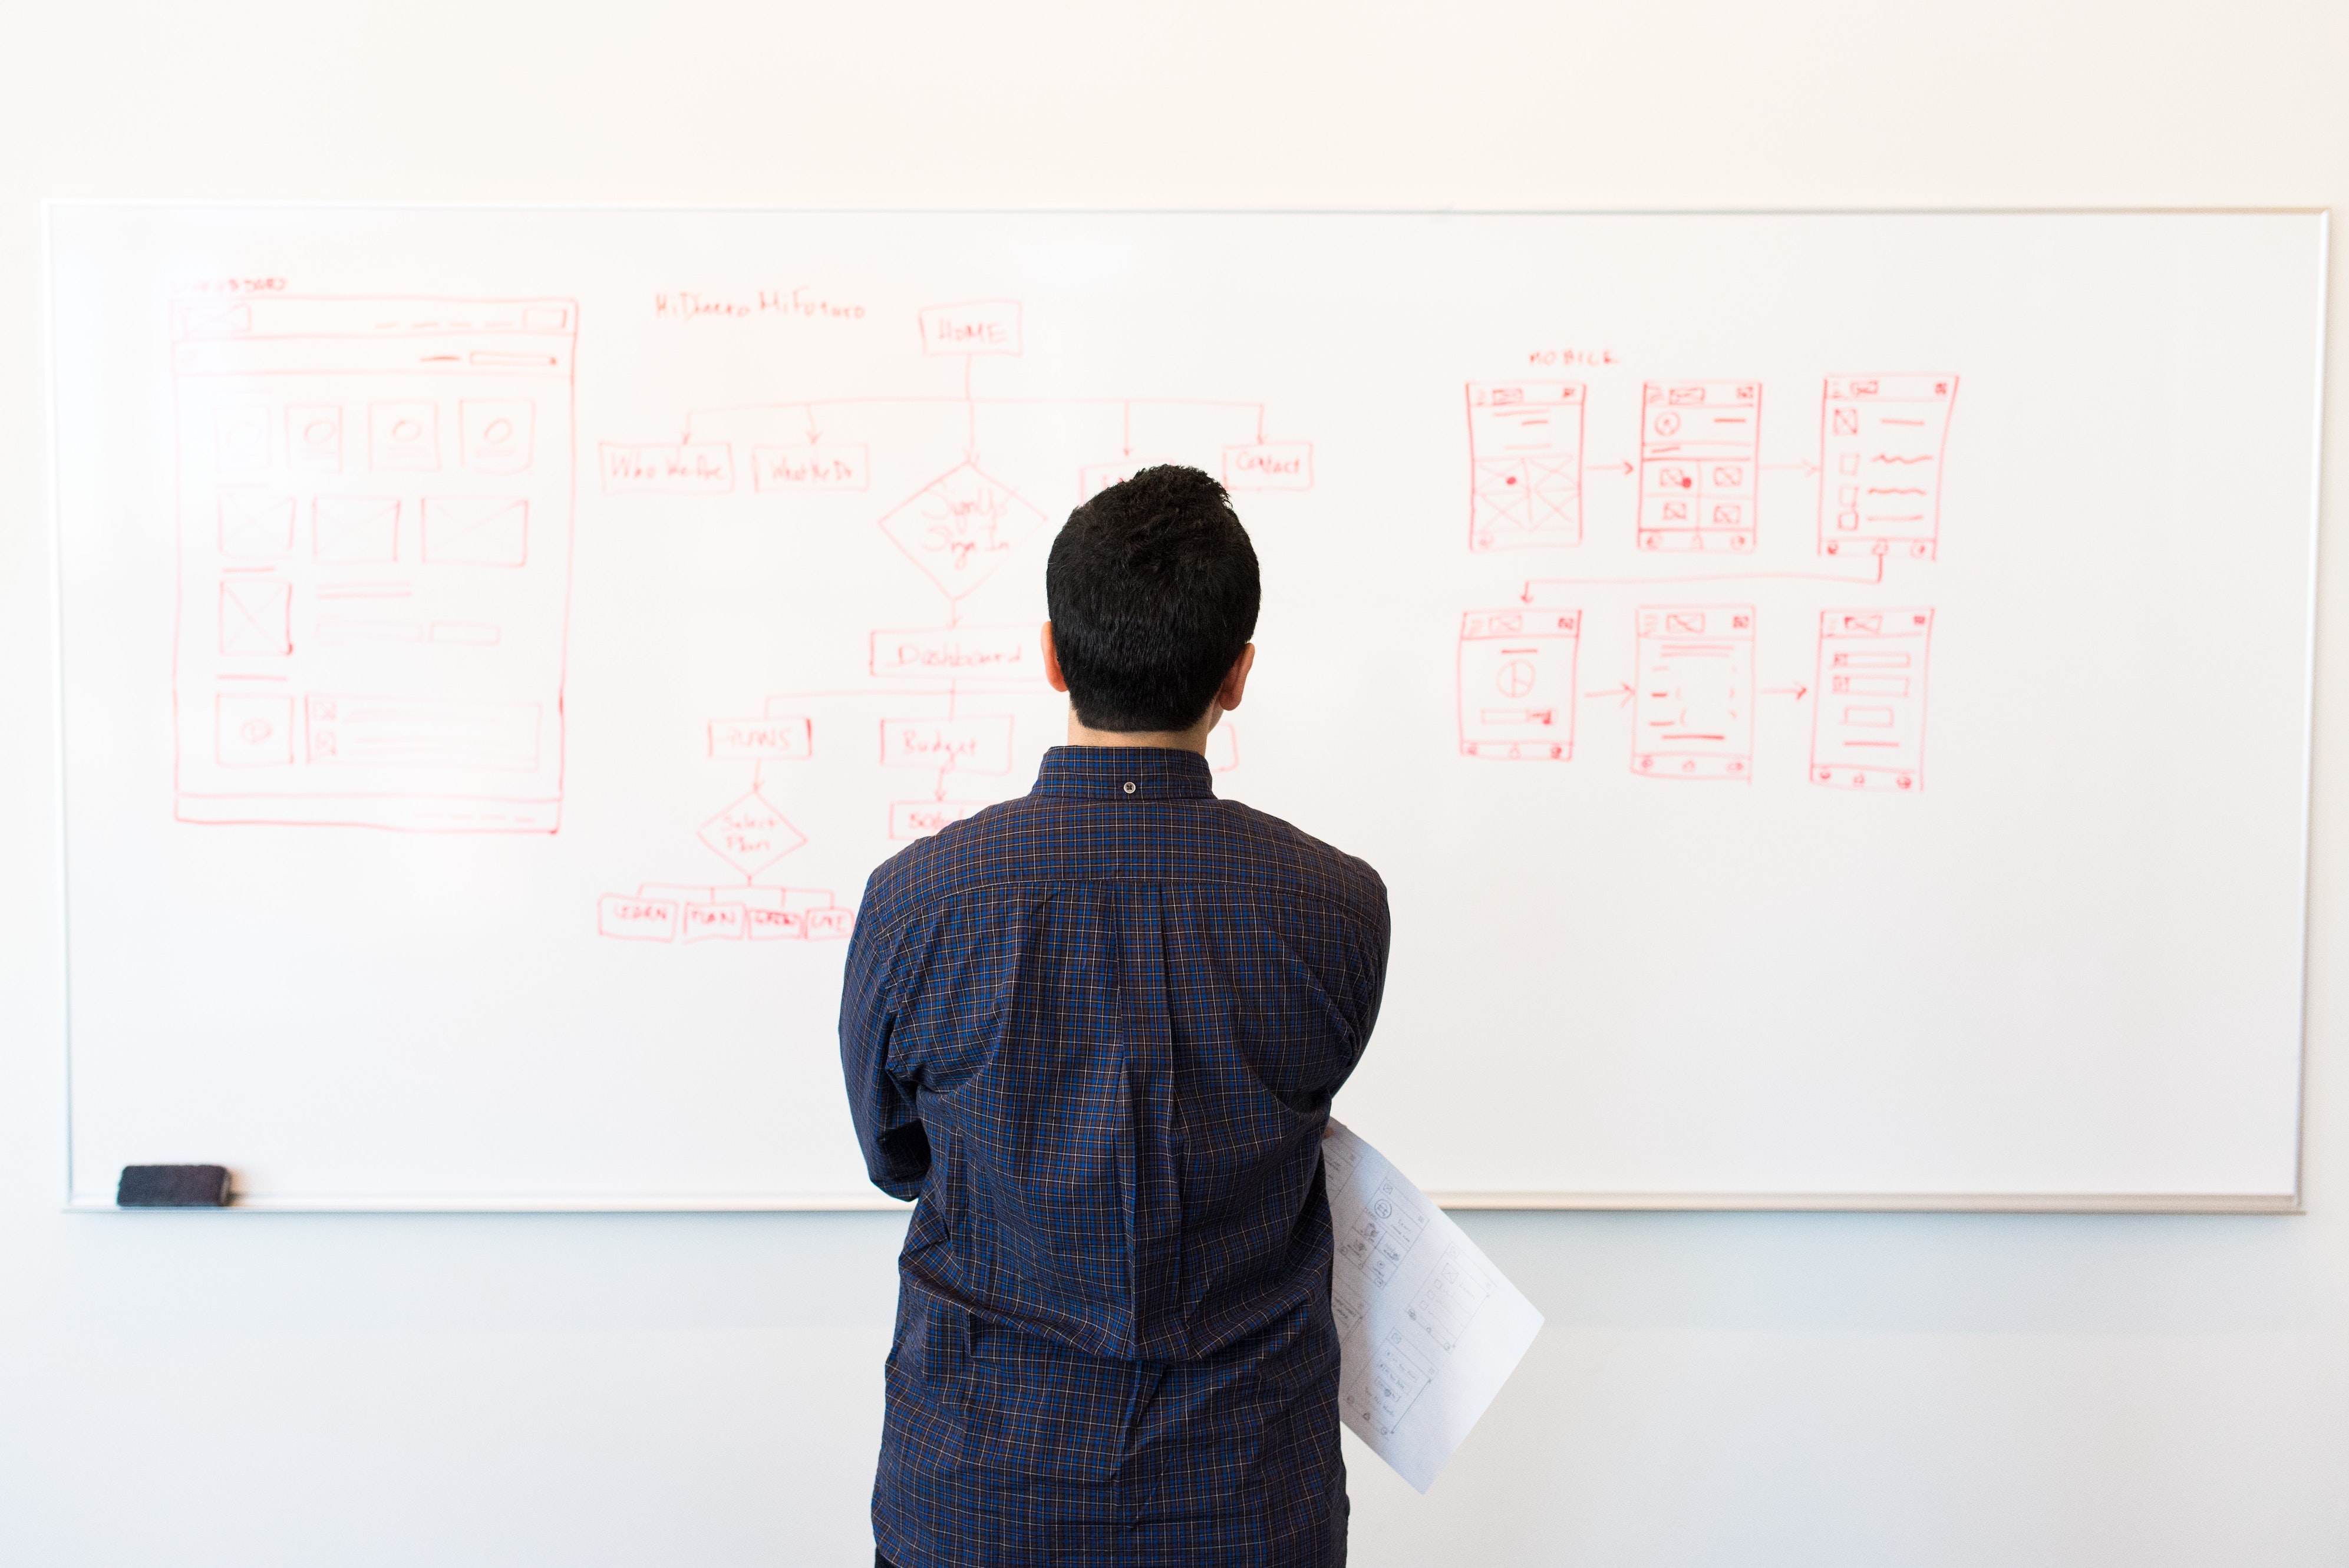
\includegraphics{C:/Users/Admin/Documents/R/WORKING_DIRECTORY/Meta-Analyse\%20Buch/bookdown-demo-master/chappool.jpg}
\caption{}
\end{figure}

\begin{rmdinfo}
This chapter will tell you about how you can \textbf{import} your effect
size data in RStudio. We will also show you a few commands which make it
easier to \textbf{manipulate data} directly in R.

Data preparation can be tedious and exhausting at times, but it is the
backbone of all later steps when doing meta-analyses in R. We therefore
have to pay close attention to preparing the data correctly before we
can proceed.
\end{rmdinfo}

\section{Data preparation in Excel}\label{data-preparation-in-excel}

\hypertarget{excel_preparation}{\subsection{Setting the columns of excel
spreadsheet}\label{excel_preparation}}

To conduct Meta-Analyses in R, you need to have your study data
prepared. For a standard meta-analysis, the following information is
needed for every study.

\begin{itemize}
\tightlist
\item
  The \textbf{names} of the individual studies, so that the can be
  easily identified later on. Usually, the first author of a study is
  used for this (e.g. ``Ebert et al., 2018'')
\item
  The \textbf{Mean} of both the Intervention and the Control group at
  the same assessment point
\item
  The \textbf{Standard Deviation} of both the Intervention and the
  Control group at the same assessment point
\item
  The \textbf{number of participants (N)} in each group of the trial
\item
  If you want to have a look at differences between various study
  subgroups later on, you also need a \textbf{subgroup code} for each
  study which signifies to which subgroup it belongs. For example, if a
  study was conducted in children, you might give it the subgroup code
  ``children''.
\end{itemize}

As per usual, such data is stored in \textbf{EXCEL spreadsheets}. We
recommend to store your data there, because this makes it very easy to
import data into RStudio.

However, it is very important how you \textbf{name the columns of your
spreadsheet}. If you name the columns of your sheet adequately in EXCEL
already, you can save a lot of time because your data doesn't have to be
transformed in RStudio later on.

\textbf{Here is how you should name the data columns in your EXCEL
spreadheet containing your Meta-Analysis data}

\begin{tabular}{l|l}
\hline
Column & Description\\
\hline
Author & This signifies the column for the study label (i.e., the first author)\\
\hline
Me & The Mean of the experimental/intervention group\\
\hline
Se & The Standard Deviation of the experimental/intervention group\\
\hline
Mc & The Mean of the control group\\
\hline
Sc & The Standard Deviation of the control group\\
\hline
Ne & The number of participants in the experimental/intervention group\\
\hline
Nc & The number of participats in the control group\\
\hline
Subgroup & This is the label for one of your Subgroup codes. It's not that important how you name it, so you can give it a more informative name (e.g. population). In this column, each study should then be given an subgroup code, which should be exactly the same for each subgroup, including upper/lowercase letters. Of course, you can also include more than one subgroup column with different subgroup codings, but the column name has to be unique\\
\hline
\end{tabular}

Note that it \textbf{doesn't matter how these columns are ordered in
your EXCEL spreadsheet}. They just have to be labeled correctly.

There's also no need to \textbf{format} the columns in any way. If you
type the column name in the first line of you spreadsheet, R will
automatically detect it as a column name.

\begin{rmdachtung}
It's also important to know that the import \textbf{will distort letters
like ä,ü,ö,á,é,ê, etc}. So be sure to transform them to ``normal''
letters before you proceed.
\end{rmdachtung}

\subsection{Setting the columns of your sheet if you have calculated the
effect sizes of each study
already}\label{setting-the-columns-of-your-sheet-if-you-have-calculated-the-effect-sizes-of-each-study-already}

If you have \textbf{already calculated the effect sizes for each study
on your own}, for example using Comprehensive Meta-Analysis or RevMan,
there's another way to prepare your data which makes things a little
easier. In this case, you only have to include the following columns:

\begin{tabular}{l|l}
\hline
Column & Description\\
\hline
Author & This signifies the column for the study label (i.e., the first author)\\
\hline
TE & The calculated effect size of the study (either Cohen's d or Hedges' g, or some other form of effect size\\
\hline
seTE & The Standard Error (SE) of the calculated effect\\
\hline
Subgroup & This is the label for one of your Subgroup codes. It's not that important how you name it, so you can give it a more informative name (e.g. population). In this column, each study should then be given an subgroup code, which should be exactly the same for each subgroup, including upper/lowercase letters. Of course, you can also include more than one subgroup column with different subgroup codings, but the column name has to be unique\\
\hline
\end{tabular}

\hypertarget{import_excel}{\section{Importing the Spreadsheet into
Rstudio}\label{import_excel}}

To get our data into R, we need to \textbf{save our data in a format and
at a place where RStudio can open it}.

\subsection{Saving the data in the right
format}\label{saving-the-data-in-the-right-format}

Generelly, finding the right format to import EXCEL can be tricky.

\begin{itemize}
\tightlist
\item
  If you're using a PC or Mac, it is advised to save your EXCEL sheet as
  a \textbf{comma-separated-values (.csv) file}. This can be done by
  clicking on ``save as'' and then choosing (.csv) as the output format.
\item
  With some PCs, RStudios might not be able to open such files, or the
  files might be distorted. In this case, you can also try to save the
  sheet as a normal \textbf{.xslx} EXCEL-file and try if this works.
\end{itemize}

\subsection{Saving the data in your working
directory}\label{saving-the-data-in-your-working-directory}

To function properly, you have to set a working directory for RStudio
first. The working directory is a \textbf{folder on your computer from
which RStudio can use data, and in which output it saved}.

\begin{enumerate}
\def\labelenumi{\arabic{enumi}.}
\tightlist
\item
  Therefore, create a folder on your computer and give it a meaningful
  name (e.g. ``My Meta-Analysis'').
\item
  Save your spreadsheet in the folder
\item
  Set the folder as your working directory. This can be done in RStudio
  on the \textbf{bottom-right corner of your screen}. Under the tile
  \textbf{``Files''}, search for the folder on your computer, and open
  it.
\item
  Once you've opened your folder, the file you just saved there should
  be in there.
\item
  Now that you've opened the folder, click on the \textbf{little gear
  wheel on top of the pane}
\end{enumerate}

\includegraphics{Doing_Meta_Analysis_in_R_files/figure-latex/unnamed-chunk-14-1.pdf}

\begin{enumerate}
\def\labelenumi{\arabic{enumi}.}
\setcounter{enumi}{5}
\tightlist
\item
  Then click on ``\textbf{Set as working directory}''
\end{enumerate}

\textbf{Your file, and the working directory, are now where they should
be!}

\subsection{Loading the data}\label{loading-the-data}

\begin{enumerate}
\def\labelenumi{\arabic{enumi}.}
\tightlist
\item
  To import the data, simply \textbf{click on the file} in the
  bottom-right pane. Then click on \textbf{import dataset\ldots{}}
\item
  An import assistant should now pop up, which is also loading a preview
  for data. This can be time consuming sometimes, so you can skip this
  step if you want to, and klick straight on \textbf{``import''}
\end{enumerate}

\includegraphics{Doing_Meta_Analysis_in_R_files/figure-latex/unnamed-chunk-15-1.pdf}

As you can see, the on the top-right pane \textbf{Environment}, your
file is now listed as a data set in your RStudio environment.

\begin{enumerate}
\def\labelenumi{\arabic{enumi}.}
\setcounter{enumi}{2}
\tightlist
\item
  I also want to give my data a shorter name (``madata''). To rename it,
  i use the following code:
\end{enumerate}

\begin{Shaded}
\begin{Highlighting}[]
\NormalTok{madata<-Meta_Analysis_Data}
\end{Highlighting}
\end{Shaded}

\begin{enumerate}
\def\labelenumi{\arabic{enumi}.}
\setcounter{enumi}{3}
\tightlist
\item
  Now, let's have a look at the \textbf{structure of my data} using the
  \texttt{str()} function
\end{enumerate}

\begin{Shaded}
\begin{Highlighting}[]
\KeywordTok{str}\NormalTok{(madata)}
\end{Highlighting}
\end{Shaded}

\begin{verbatim}
## Classes 'tbl_df', 'tbl' and 'data.frame':    18 obs. of  17 variables:
##  $ Author               : chr  "Call et al." "Cavanagh et al." "DanitzOrsillo" "de Vibe et al." ...
##  $ TE                   : num  0.709 0.355 1.791 0.182 0.422 ...
##  $ seTE                 : num  0.261 0.196 0.346 0.118 0.145 ...
##  $ RoB                  : chr  "low" "low" "high" "low" ...
##  $ Control              : chr  "WLC" "WLC" "WLC" "no intervention" ...
##  $ intervention duration: chr  "short" "short" "short" "short" ...
##  $ intervention type    : chr  "mindfulness" "mindfulness" "ACT" "mindfulness" ...
##  $ population           : chr  "undergraduate students" "students" "undergraduate students" "undergraduate students" ...
##  $ type of students     : chr  "psychology" "general" "general" "general" ...
##  $ prevention type      : chr  "selective" "universal" "universal" "universal" ...
##  $ gender               : chr  "female" "mixed" "mixed" "mixed" ...
##  $ mode of delivery     : chr  "group" "online" "group" "group" ...
##  $ ROB streng           : chr  "high" "low" "high" "low" ...
##  $ ROB superstreng      : chr  "high" "high" "high" "low" ...
##  $ compensation         : chr  "none" "none" "voucher/money" "voucher/money" ...
##  $ instruments          : chr  "DASS" "PSS" "DASS" "other" ...
##  $ guidance             : chr  "f2f" "self-guided" "f2f" "f2f" ...
\end{verbatim}

Although this output looks kind of messy, it's already very informative.
It shows the structure of my data. In this case, i used data for which
the effect sizes were already calculated. This is why the variables
\textbf{TE} and \textbf{seTE} appear. I also see plenty of other
variables, which correspond to the subgroups which were coded for this
dataset.

\textbf{Here's a (shortened) table created for my data}

\begin{tabular}{l|r|r|l|l|l|l}
\hline
Author & TE & seTE & RoB & Control & intervention duration & intervention type\\
\hline
Call et al. & 0.7091362 & 0.2608202 & low & WLC & short & mindfulness\\
\hline
Cavanagh et al. & 0.3548641 & 0.1963624 & low & WLC & short & mindfulness\\
\hline
DanitzOrsillo & 1.7911700 & 0.3455692 & high & WLC & short & ACT\\
\hline
de Vibe et al. & 0.1824552 & 0.1177874 & low & no intervention & short & mindfulness\\
\hline
Frazier et al. & 0.4218509 & 0.1448128 & low & information only & short & PCI\\
\hline
Frogeli et al. & 0.6300000 & 0.1960000 & low & no intervention & short & ACT\\
\hline
Gallego et al. & 0.7248838 & 0.2246641 & high & no intervention & long & mindfulness\\
\hline
Hazlett-Stevens \& Oren & 0.5286638 & 0.2104609 & low & no intervention & long & mindfulness\\
\hline
Hintz et al. & 0.2840000 & 0.1680000 & low & information only & short & PCI\\
\hline
Kang et al. & 1.2750682 & 0.3371997 & low & no intervention & long & mindfulness\\
\hline
Kuhlmann et al. & 0.1036082 & 0.1947275 & low & no intervention & short & mindfulness\\
\hline
Lever Taylor et al. & 0.3883906 & 0.2307689 & low & WLC & long & mindfulness\\
\hline
Phang et al. & 0.5407398 & 0.2443133 & low & no intervention & short & mindfulness\\
\hline
Rasanen et al. & 0.4261593 & 0.2579379 & low & WLC & short & ACT\\
\hline
Ratanasiripong & 0.5153969 & 0.3512737 & high & no intervention & short & mindfulness\\
\hline
Shapiro et al. & 1.4797260 & 0.3152817 & low & WLC & long & mindfulness\\
\hline
SongLindquist & 0.6125782 & 0.2266834 & high & WLC & long & mindfulness\\
\hline
Warnecke et al. & 0.6000000 & 0.2490000 & low & information only & long & mindfulness\\
\hline
\end{tabular}

\section{Data manipulation}\label{data-manipulation}

Now that we have the Meta-Analysis data in RStudio, let's do a few
manipulations with the data. These functions might come in handy when
were conducting analyses later on.

Going back to the output of the \texttt{str()} function, we see that
this also gives us details on the type of column data we have stored in
our data. There a different abbreviations signifying different types of
data.

\begin{tabular}{l|l|l}
\hline
Abbreviation & Type & Description\\
\hline
num & Numerical & This is all data stored as numbers (e.g. 1.02)\\
\hline
chr & Character & This is all data stored as words\\
\hline
log & Logical & These are variables which are binary, meaning that they signify that a condition is either TRUE or FALSE\\
\hline
factor & Factor & Factors are stored as numbers, with each number signifying a different level of a variable. A possible factor of a variable might be 1 = low, 2 = medium, 3 = high\\
\hline
\end{tabular}

\subsection{Converting to factors}\label{converting-to-factors}

Let's say we have the subgroup \textbf{Risk of Bias} (in which the Risk
of Bias rating is coded), and want it to be a factor with two different
levels: ``low'' and ``high''.

To do this, we need to the variable \texttt{ROB} to be a factor.
However, this variable is currently stored as a character
(\texttt{chr}). We can have a look at this variable by typing the name
of our dataset, then adding the selector \texttt{\$} and then adding the
variable we want to have a look at.

\begin{Shaded}
\begin{Highlighting}[]
\NormalTok{madata}\OperatorTok{$}\NormalTok{ROB}
\end{Highlighting}
\end{Shaded}

\begin{verbatim}
##  [1] "high" "low"  "high" "low"  "low"  "low"  "high" "low"  "low"  "low" 
## [11] "high" "low"  "low"  "low"  "high" "high" "high" "low"
\end{verbatim}

\begin{Shaded}
\begin{Highlighting}[]
\KeywordTok{str}\NormalTok{(madata}\OperatorTok{$}\NormalTok{ROB)}
\end{Highlighting}
\end{Shaded}

\begin{verbatim}
##  chr [1:18] "high" "low" "high" "low" "low" "low" "high" "low" "low" ...
\end{verbatim}

We can see now that \texttt{ROB}is indeed a \textbf{character} type
variable, which contains only to words: ``low'' and ``high''. We want to
convert this to a \textbf{factor} variable now, which has only two
levels, low and high. To do this, we use the \texttt{as.factor()}
function.

\begin{Shaded}
\begin{Highlighting}[]
\NormalTok{madata}\OperatorTok{$}\NormalTok{ROB<-}\KeywordTok{factor}\NormalTok{(madata}\OperatorTok{$}\NormalTok{ROB)}
\NormalTok{madata}\OperatorTok{$}\NormalTok{ROB}
\end{Highlighting}
\end{Shaded}

\begin{verbatim}
##  [1] high low  high low  low  low  high low  low  low  high low  low  low 
## [15] high high high low 
## Levels: high low
\end{verbatim}

\begin{Shaded}
\begin{Highlighting}[]
\KeywordTok{str}\NormalTok{(madata}\OperatorTok{$}\NormalTok{ROB)}
\end{Highlighting}
\end{Shaded}

\begin{verbatim}
##  Factor w/ 2 levels "high","low": 1 2 1 2 2 2 1 2 2 2 ...
\end{verbatim}

We now see that the variable has been \textbf{converted to a factor with
the levels ``high'' and ``low''}.

\subsection{Converting to logicals}\label{converting-to-logicals}

Now lets have a look at the \textbf{intervention type} subgroup
variable. This variable is corrently stores as a character too.

\begin{Shaded}
\begin{Highlighting}[]
\NormalTok{madata}\OperatorTok{$}\StringTok{`}\DataTypeTok{intervention type}\StringTok{`}
\end{Highlighting}
\end{Shaded}

\begin{verbatim}
##  [1] "mindfulness" "mindfulness" "ACT"         "mindfulness" "PCI"        
##  [6] "ACT"         "mindfulness" "mindfulness" "PCI"         "mindfulness"
## [11] "mindfulness" "mindfulness" "mindfulness" "ACT"         "mindfulness"
## [16] "mindfulness" "mindfulness" "mindfulness"
\end{verbatim}

\begin{Shaded}
\begin{Highlighting}[]
\KeywordTok{str}\NormalTok{(madata}\OperatorTok{$}\StringTok{`}\DataTypeTok{intervention type}\StringTok{`}\NormalTok{)}
\end{Highlighting}
\end{Shaded}

\begin{verbatim}
##  chr [1:18] "mindfulness" "mindfulness" "ACT" "mindfulness" "PCI" ...
\end{verbatim}

Let's say we want a variable which only contains information if a study
way a mindfulness intervention or not. A logical is very well suited for
this. To convert the data to logical, we use the \texttt{as.logical}
function. We will create a new variable containing this information
called \texttt{intervention.type.logical}. To tell R what to count as
\texttt{TRUE} and what as \texttt{FALSE}, we have to define the specific
intervention type using the \texttt{==} command.

\begin{Shaded}
\begin{Highlighting}[]
\NormalTok{intervention.type.logical<-}\KeywordTok{as.logical}\NormalTok{(madata}\OperatorTok{$}\StringTok{`}\DataTypeTok{intervention type}\StringTok{`}\OperatorTok{==}\StringTok{"mindfulness"}\NormalTok{)}
\NormalTok{intervention.type.logical}
\end{Highlighting}
\end{Shaded}

\begin{verbatim}
##  [1]  TRUE  TRUE FALSE  TRUE FALSE FALSE  TRUE  TRUE FALSE  TRUE  TRUE
## [12]  TRUE  TRUE FALSE  TRUE  TRUE  TRUE  TRUE
\end{verbatim}

We see that R has converted the character information into trues and
falses for us. To check if this was done correctly, let's compare the
original and the new variable

\begin{Shaded}
\begin{Highlighting}[]
\NormalTok{n<-}\KeywordTok{data.frame}\NormalTok{(intervention.type.logical,madata}\OperatorTok{$}\StringTok{`}\DataTypeTok{intervention type}\StringTok{`}\NormalTok{)}
\NormalTok{names<-}\KeywordTok{c}\NormalTok{(}\StringTok{"New"}\NormalTok{, }\StringTok{"Original"}\NormalTok{)}
\KeywordTok{colnames}\NormalTok{(n)<-names}
\KeywordTok{kable}\NormalTok{(n)}
\end{Highlighting}
\end{Shaded}

\begin{tabular}{l|l}
\hline
New & Original\\
\hline
TRUE & mindfulness\\
\hline
TRUE & mindfulness\\
\hline
FALSE & ACT\\
\hline
TRUE & mindfulness\\
\hline
FALSE & PCI\\
\hline
FALSE & ACT\\
\hline
TRUE & mindfulness\\
\hline
TRUE & mindfulness\\
\hline
FALSE & PCI\\
\hline
TRUE & mindfulness\\
\hline
TRUE & mindfulness\\
\hline
TRUE & mindfulness\\
\hline
TRUE & mindfulness\\
\hline
FALSE & ACT\\
\hline
TRUE & mindfulness\\
\hline
TRUE & mindfulness\\
\hline
TRUE & mindfulness\\
\hline
TRUE & mindfulness\\
\hline
\end{tabular}

\subsection{Selecting specific
studies}\label{selecting-specific-studies}

It may often come in handy to \textbf{select certain studies for further
analyses}, or to \textbf{exclude some studies in further analyses}
(e.g., if they are outliers).

To do this, we can use the \texttt{filter} function in the
\texttt{dplyr}package, which is part of the \texttt{tidyverse} package
we installed before.

So, let's load the package first.

\begin{Shaded}
\begin{Highlighting}[]
\KeywordTok{library}\NormalTok{(dplyr)}
\end{Highlighting}
\end{Shaded}

Let's say we want to do a Meta-Analysis with three studies in our
dataset only. To do this, we need to create a new dataset containing
only these studies using the \texttt{dplyr::filter()} function. The
\texttt{dplyr::} part is necessary as there a more than one filter
functions in R, and we want to use to use the one of the
\texttt{dplyr}package.

Let's say we want to have the studies by \textbf{Cavanagh et al.},
\textbf{Frazier et al.} and \textbf{Phang et al.} stored in another
dataset, so we can conduct analyses only for these studies.

The R code to store theses three studies in a new dataset called
\texttt{madata.new} looks like this:

\begin{Shaded}
\begin{Highlighting}[]
\NormalTok{madata.new<-dplyr}\OperatorTok{::}\KeywordTok{filter}\NormalTok{(madata,Author }\OperatorTok\StringTok{ }\KeywordTok{c}\NormalTok{(}\StringTok{"Cavanagh et al."}\NormalTok{,}\StringTok{"Frazier et al."}\NormalTok{,}\StringTok{"Phang et al."}\NormalTok{))}
\end{Highlighting}
\end{Shaded}

Note that the \texttt{\%in\%}-Command tells the \texttt{filter} function
to search for exactly the three cases we defined in the variable
\texttt{Author}. Now, let's have a look at the new data
\texttt{madata.new} we just created.

\begin{tabular}{l|r|r|l|l|l|l|l|l|l|l|l|l|l|l|l|l|l}
\hline
Author & TE & seTE & RoB & Control & intervention duration & intervention type & population & type of students & prevention type & gender & mode of delivery & ROB streng & ROB superstreng & compensation & instruments & guidance & ROB\\
\hline
Cavanagh et al. & 0.3548641 & 0.1963624 & low & WLC & short & mindfulness & students & general & universal & mixed & online & low & high & none & PSS & self-guided & low\\
\hline
Frazier et al. & 0.4218509 & 0.1448128 & low & information only & short & PCI & students & psychology & universal & mixed & online & low & low & credit & PSS & reminders & low\\
\hline
Phang et al. & 0.5407398 & 0.2443133 & low & no intervention & short & mindfulness & students & medical studens & selective & mixed & group & low & low & none & PSS & f2f & low\\
\hline
\end{tabular}

Note that the function can also be used for any other type of data and
variable. We can also use it to e.g., only select studies which were
coded as being a mindfulness study

\begin{Shaded}
\begin{Highlighting}[]
\NormalTok{madata.new.mf<-dplyr}\OperatorTok{::}\KeywordTok{filter}\NormalTok{(madata,}\StringTok{`}\DataTypeTok{intervention type}\StringTok{`} \OperatorTok\StringTok{ }\KeywordTok{c}\NormalTok{(}\StringTok{"mindfulness"}\NormalTok{))}
\end{Highlighting}
\end{Shaded}

We can also use the \texttt{dplyr::filter()} function to exclude studies
from our dataset. To do this, we only have to add \texttt{!} in front of
the variable we want to use for filtering.

\begin{Shaded}
\begin{Highlighting}[]
\NormalTok{madata.new.excl<-dplyr}\OperatorTok{::}\KeywordTok{filter}\NormalTok{(madata,}\OperatorTok{!}\NormalTok{Author }\OperatorTok\StringTok{ }\KeywordTok{c}\NormalTok{(}\StringTok{"Cavanagh et al."}\NormalTok{,}\StringTok{"Frazier et al."}\NormalTok{,}\StringTok{"Phang et al."}\NormalTok{))}
\end{Highlighting}
\end{Shaded}

\subsection{Changing cell values}\label{changing-cell-values}

Sometimes, even when preparing your data in EXCEL, you might want to
\textbf{change values in RStudio once you have imported your data}.

To do this, we have to select a cell in our data frame in RStudio. This
can be done by adding \texttt{{[}x,y{]}} to our dataset name, where
\textbf{x} signifies the number of the \textbf{row} we want to select,
and \textbf{y} signifies the number of the \textbf{column}.

To see how this works, let's select a variable using this command first:

\begin{Shaded}
\begin{Highlighting}[]
\NormalTok{madata[}\DecValTok{6}\NormalTok{,}\DecValTok{1}\NormalTok{]}
\end{Highlighting}
\end{Shaded}

\begin{verbatim}
## # A tibble: 1 x 1
##   Author        
##   <chr>         
## 1 Frogeli et al.
\end{verbatim}

We now see the \textbf{6th study} in our dataframe, and the value of
this study for \textbf{Column 1 (the author name)} is displayed. Let's
say we had a typo in this name and want to have it changed. In this
case, we have to give this exact cell a new value.

\begin{Shaded}
\begin{Highlighting}[]
\NormalTok{madata[}\DecValTok{6}\NormalTok{,}\DecValTok{1}\NormalTok{]<-}\StringTok{"Frogelli et al."}
\end{Highlighting}
\end{Shaded}

Let's check if the name has changed.

\begin{Shaded}
\begin{Highlighting}[]
\NormalTok{madata[}\DecValTok{6}\NormalTok{,}\DecValTok{1}\NormalTok{]}
\end{Highlighting}
\end{Shaded}

\begin{verbatim}
## # A tibble: 1 x 1
##   Author         
##   <chr>          
## 1 Frogelli et al.
\end{verbatim}

You can also use this function to change any other type of data,
including numericals and logicals. Only for characters, you have to put
the values you want to insert in \texttt{""}.

\chapter{Pooling Effect Sizes}\label{pool}

\begin{figure}
\centering
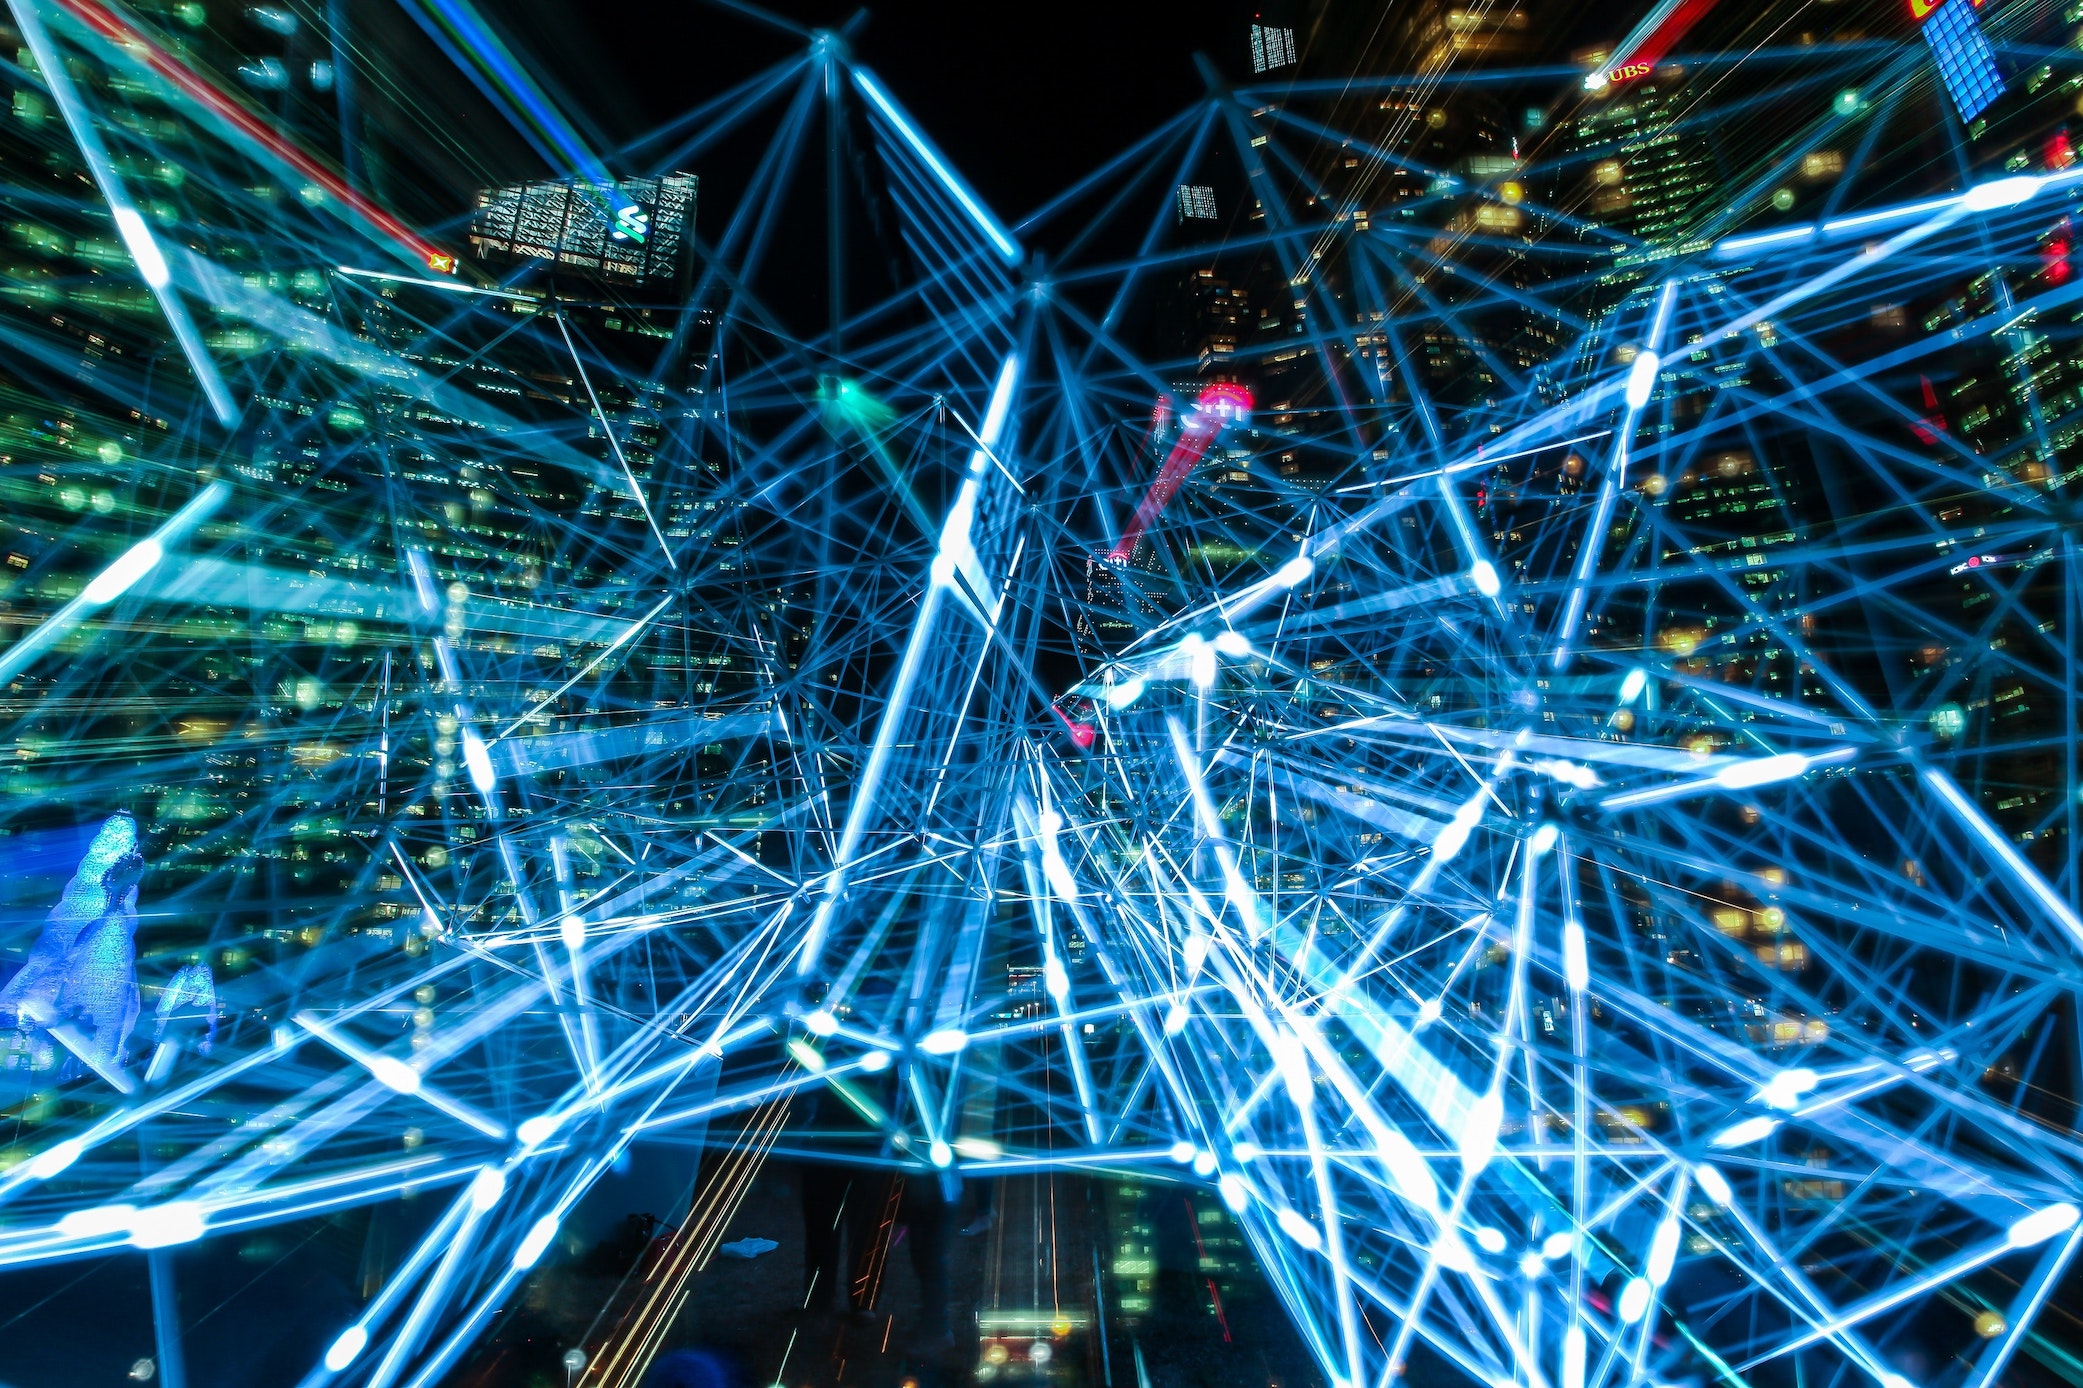
\includegraphics{C:/Users/Admin/Documents/R/WORKING_DIRECTORY/Meta-Analyse\%20Buch/bookdown-demo-master/pooling.jpg}
\caption{}
\end{figure}

Now, let's get to the core of every Meta-Analysis: \textbf{pooling your
effect sizes} to get one overall effect size estimate of the studies.

\begin{rmdinfo}
When pooling effect sizes in Meta-Analysis, there are two approaches
which we can use: the \textbf{Fixed-Effects-Model}, or the
\textbf{Random-Effects-Model} {[}@borenstein2011{]}. There is an
extensive debate on which model fits best in which context
{[}@fleiss1993review{]}, with no clear consensus in sight. Although it
has been recommended to \textbf{only resort to the
Random-Effects-Pooling model} in clinical psychology and the health
sciences {[}@cuijpers2016meta{]}, we will describe how to conduct both
in R here.

Both of these models only require an \textbf{effect size}, and a
\textbf{dispersion (variance)} estimate for each study, of which the
inverse is taken. This is why the methods are often called
\textbf{general inverse-variance methods}.
\end{rmdinfo}

We will describe in-depth how to conduct meta-analyses in R with
\textbf{continuous variables} (such as effect sizes), as these are the
most common ones in psychology and the health science field. Later on,
we will present briefly how to do meta-analyses with \textbf{binary
outcome} data too, which might be important if you're focusing on
prevention trials.

For these Meta-Analyses, we'll use the \texttt{meta} package
\citep{schwarzer2007meta}. In \protect\hyperlink{RStudio}{Section 2.1},
we show how to install the package. Now, load the package from your
library to proceed.

\begin{Shaded}
\begin{Highlighting}[]
\KeywordTok{library}\NormalTok{(meta)}
\end{Highlighting}
\end{Shaded}

\hypertarget{fixed}{\section{Fixed-Effects-Model}\label{fixed}}

\subsection{Pre-calculated effect size
data}\label{pre-calculated-effect-size-data}

\begin{rmdinfo}
\textbf{The idea behind the fixed-effects-model}

The fixed-effects-model assumes that all studies along with their effect
sizes stem from a single homogeneous population {[}@borenstein2011{]}.
To calculate the overall effect, we therefore average all effect sizes,
but give studies with greater precision a higher weight. In this case,
greater precision means that the study has a larger \textbf{N}, which
leads to a smaller \textbf{Standard Error} of its effect size estimate.

For this weighing, we use the \textbf{inverse of the variance}
\(1/\hat\sigma^2_k\) of each study \(k\). We then calculate a weighted
average of all studies, our fixed effect size estimator
\(\hat\theta_F\):
\end{rmdinfo}

\begin{equation}
\hat\theta_F = \frac{\sum\limits_{k=1}^K \hat\theta_k/ \hat\sigma^2_k}{\sum\limits_{k=1}^K 1/\hat\sigma^2_k}
\end{equation}

In \protect\hyperlink{excel_preparation}{Chapter 3.1}, we have described
two ways your EXCEL spreadsheet for you Meta-Analysis data can look
like:

\begin{itemize}
\tightlist
\item
  It can either be stored as the raw data (including the Mean, N, and SD
  of every study arm)
\item
  Or it only contains the calculated effect sizes and the standard error
  (SE)
\end{itemize}

The functions to pool the results with a fixed-effects-model differ
depending on which data format you used, but not much. First, let's
assume you already have a dataset with the calucated effects and SE for
each study. In my case, this is my \texttt{madata} dataset.

\begin{Shaded}
\begin{Highlighting}[]
\KeywordTok{str}\NormalTok{(madata)}
\end{Highlighting}
\end{Shaded}

\begin{verbatim}
## Classes 'tbl_df', 'tbl' and 'data.frame':    18 obs. of  17 variables:
##  $ Author               : chr  "Call et al." "Cavanagh et al." "DanitzOrsillo" "de Vibe et al." ...
##  $ TE                   : num  0.709 0.355 1.791 0.182 0.422 ...
##  $ seTE                 : num  0.261 0.196 0.346 0.118 0.145 ...
##  $ RoB                  : chr  "low" "low" "high" "low" ...
##  $ Control              : chr  "WLC" "WLC" "WLC" "no intervention" ...
##  $ intervention duration: chr  "short" "short" "short" "short" ...
##  $ intervention type    : chr  "mindfulness" "mindfulness" "ACT" "mindfulness" ...
##  $ population           : chr  "undergraduate students" "students" "undergraduate students" "undergraduate students" ...
##  $ type of students     : chr  "psychology" "general" "general" "general" ...
##  $ prevention type      : chr  "selective" "universal" "universal" "universal" ...
##  $ gender               : chr  "female" "mixed" "mixed" "mixed" ...
##  $ mode of delivery     : chr  "group" "online" "group" "group" ...
##  $ ROB streng           : chr  "high" "low" "high" "low" ...
##  $ ROB superstreng      : chr  "high" "high" "high" "low" ...
##  $ compensation         : chr  "none" "none" "voucher/money" "voucher/money" ...
##  $ instruments          : chr  "DASS" "PSS" "DASS" "other" ...
##  $ guidance             : chr  "f2f" "self-guided" "f2f" "f2f" ...
\end{verbatim}

This dataset has \textbf{continuous outcome data}. As our effect sizes
are already calculated, we can use the \texttt{meta::metagen} function.
For this function, we can specify loads of parameters, all of which you
can access by typing \texttt{?metagen} in your console once the
\texttt{meta} package is loaded.

Here is a table with the most important parameters for our code:

\begin{tabular}{l|l}
\hline
Parameter & Function\\
\hline
TE & This tells R to use the TE column to retrieve the effect sizes for each study\\
\hline
seTE & This tells R to use the seTE column to retrieve the standard error for each             study\\
\hline
data= & After =, paste the name of your dataset here\\
\hline
studlab=paste() & This tells the function were the labels for each study are stored. If you named the spreadsheet columns as advised, this should be studlab=paste(Author)\\
\hline
comb.fixed= & Weather to use a fixed-effects-model\\
\hline
comb.random & Weather to use a random-effects-model\\
\hline
prediction= & Weather to print a prediction interval for the effect of future studies based on present evidence\\
\hline
sm= & The summary measure we want to calculate. We can either calculate the mean difference (MD) or Hedges' g (SMD)\\
\hline
\end{tabular}

Let's code our first fixed-effects-model Meta-Analysis. We we will give
the results of this analysis the simple name \texttt{m}.

\begin{Shaded}
\begin{Highlighting}[]
\NormalTok{m<-}\KeywordTok{metagen}\NormalTok{(TE,}
\NormalTok{        seTE,}
        \DataTypeTok{data=}\NormalTok{madata,}
        \DataTypeTok{studlab=}\KeywordTok{paste}\NormalTok{(Author),}
        \DataTypeTok{comb.fixed =} \OtherTok{TRUE}\NormalTok{,}
        \DataTypeTok{comb.random =} \OtherTok{FALSE}\NormalTok{,}
        \DataTypeTok{prediction=}\OtherTok{TRUE}\NormalTok{,}
        \DataTypeTok{sm=}\StringTok{"SMD"}\NormalTok{)}
\NormalTok{m}
\end{Highlighting}
\end{Shaded}

\begin{verbatim}
##                           SMD            95%-CI %W(fixed)
## Call et al.            0.7091 [ 0.1979; 1.2203]       3.6
## Cavanagh et al.        0.3549 [-0.0300; 0.7397]       6.3
## DanitzOrsillo          1.7912 [ 1.1139; 2.4685]       2.0
## de Vibe et al.         0.1825 [-0.0484; 0.4133]      17.5
## Frazier et al.         0.4219 [ 0.1380; 0.7057]      11.6
## Frogeli et al.         0.6300 [ 0.2458; 1.0142]       6.3
## Gallego et al.         0.7249 [ 0.2846; 1.1652]       4.8
## Hazlett-Stevens & Oren 0.5287 [ 0.1162; 0.9412]       5.5
## Hintz et al.           0.2840 [-0.0453; 0.6133]       8.6
## Kang et al.            1.2751 [ 0.6142; 1.9360]       2.1
## Kuhlmann et al.        0.1036 [-0.2781; 0.4853]       6.4
## Lever Taylor et al.    0.3884 [-0.0639; 0.8407]       4.6
## Phang et al.           0.5407 [ 0.0619; 1.0196]       4.1
## Rasanen et al.         0.4262 [-0.0794; 0.9317]       3.6
## Ratanasiripong         0.5154 [-0.1731; 1.2039]       2.0
## Shapiro et al.         1.4797 [ 0.8618; 2.0977]       2.4
## SongLindquist          0.6126 [ 0.1683; 1.0569]       4.7
## Warnecke et al.        0.6000 [ 0.1120; 1.0880]       3.9
## 
## Number of studies combined: k = 18
## 
##                        SMD            95%-CI    z  p-value
## Fixed effect model  0.4805 [ 0.3840; 0.5771] 9.75 < 0.0001
## Prediction interval        [-0.0344; 1.1826]              
## 
## Quantifying heterogeneity:
## tau^2 = 0.0752; H = 1.64 [1.27; 2.11]; I^2 = 62.6% [37.9%; 77.5%]
## 
## Test of heterogeneity:
##      Q d.f. p-value
##  45.50   17  0.0002
## 
## Details on meta-analytical method:
## - Inverse variance method
\end{verbatim}

We now see the results of our Meta-Analysis, including

\begin{itemize}
\tightlist
\item
  The \textbf{individual effect sizes} for each study, and their weight
\item
  The total \textbf{number of included studies} (k)
\item
  The \textbf{overall effect} (in our case, g=0.4805) and its confidence
  interval and p-value
\item
  Measures of \textbf{between-study heterogeneity}, such as
  \emph{tau\textsuperscript{2}} or \emph{I\textsuperscript{2}} and a
  \emph{Q}-test of heterogeneity
\end{itemize}

Using the \texttt{\$} command, we can also have a look at various
outputs directly. For example

\begin{Shaded}
\begin{Highlighting}[]
\NormalTok{m}\OperatorTok{$}\NormalTok{lower.I2}
\end{Highlighting}
\end{Shaded}

Gives us the lower 95\% confidence interval for
\emph{I\textsuperscript{2}}

\begin{verbatim}
## [1] 0.3787897
\end{verbatim}

We can \textbf{save the results of the meta-analysis} to our working
directory as a .txt-file using this command

\begin{Shaded}
\begin{Highlighting}[]
\KeywordTok{sink}\NormalTok{(}\StringTok{"results.txt"}\NormalTok{)}
\KeywordTok{print}\NormalTok{(m)}
\KeywordTok{sink}\NormalTok{()}
\end{Highlighting}
\end{Shaded}

\subsection{Raw effect size data}\label{fixed.raw}

To conduct a fixed-effects-model Meta-Analysis from \textbf{raw data}
(i.e, if your data has been prepared the way we describe in
\protect\hyperlink{excel_preparation}{Chapter 3.1.1}), we have to use
the \texttt{meta::metacont()} function instead. The structure of the
code however, looks quite similar.

\begin{tabular}{l|l}
\hline
Parameter & Function\\
\hline
Ne & The number of participants (N) in the intervention group\\
\hline
Me & The Mean (M) of the intervention group\\
\hline
Se & The Standard Deviation (SD) of the intervention group\\
\hline
Nc & The number of participants (N) in the control group\\
\hline
Mc & The Mean (M) of the control group\\
\hline
Sc & The Standard Deviation (SD) of the control group\\
\hline
data= & After '=', paste the name of your dataset here\\
\hline
studlab=paste() & This tells the function were the labels for each study are stored. If you named the spreadsheet columns as advised, this should be studlab=paste(Author)\\
\hline
comb.fixed= & Weather to use a fixed-effects-model\\
\hline
comb.random & Weather to use a random-effects-model\\
\hline
prediction= & Weather to print a prediction interval for the effect of future studies based on present evidence\\
\hline
sm= & The summary measure we want to calculate. We can either calculate the mean difference (MD) or Hedges' g (SMD)\\
\hline
\end{tabular}

For this purpose, i will use my dataset \texttt{metacont}, which
contains the raw data of all studies i want to snythesize

\begin{Shaded}
\begin{Highlighting}[]
\KeywordTok{str}\NormalTok{(metacont)}
\end{Highlighting}
\end{Shaded}

\begin{verbatim}
## Classes 'tbl_df', 'tbl' and 'data.frame':    6 obs. of  7 variables:
##  $ Author: chr  "Cavanagh" "Day" "Frazier" "Gaffney" ...
##  $ Ne    : num  50 64 90 30 77 60
##  $ Me    : num  4.5 18.3 12.5 2.34 15.21 ...
##  $ Se    : num  2.7 6.4 3.2 0.87 5.35 ...
##  $ Nc    : num  50 65 95 30 69 60
##  $ Mc    : num  5.6 20.2 15.5 3.13 20.13 ...
##  $ Sc    : num  2.6 7.6 4.4 1.23 7.43 ...
\end{verbatim}

Now, let's code the Meta-Analysis function, this time using the
\texttt{meta::metacont} function, and my \texttt{metacont} dataset. I
want to name my output \texttt{m.raw} now.

\begin{Shaded}
\begin{Highlighting}[]
\NormalTok{m.raw<-}\KeywordTok{metacont}\NormalTok{(Ne,}
\NormalTok{                Me,}
\NormalTok{                Se,}
\NormalTok{                Nc,}
\NormalTok{                Mc,}
\NormalTok{                Sc,}
                \DataTypeTok{data=}\NormalTok{metacont,}
                \DataTypeTok{studlab=}\KeywordTok{paste}\NormalTok{(Author),}
                \DataTypeTok{comb.fixed =} \OtherTok{TRUE}\NormalTok{,}
                \DataTypeTok{comb.random =} \OtherTok{FALSE}\NormalTok{,}
                \DataTypeTok{prediction=}\OtherTok{TRUE}\NormalTok{,}
                \DataTypeTok{sm=}\StringTok{"SMD"}\NormalTok{)}
\NormalTok{m.raw}
\end{Highlighting}
\end{Shaded}

\begin{verbatim}
##              SMD             95%-CI %W(fixed)
## Cavanagh -0.4118 [-0.8081; -0.0155]      13.8
## Day      -0.2687 [-0.6154;  0.0781]      18.0
## Frazier  -0.7734 [-1.0725; -0.4743]      24.2
## Gaffney  -0.7303 [-1.2542; -0.2065]       7.9
## Greer    -0.7624 [-1.0992; -0.4256]      19.1
## Harrer   -0.1669 [-0.5254;  0.1916]      16.9
## 
## Number of studies combined: k = 6
## 
##                         SMD             95%-CI     z  p-value
## Fixed effect model  -0.5245 [-0.6718; -0.3773] -6.98 < 0.0001
## Prediction interval         [-1.1817;  0.1494]               
## 
## Quantifying heterogeneity:
## tau^2 = 0.0441; H = 1.51 [1.00; 2.38]; I^2 = 56.1% [0.0%; 82.3%]
## 
## Test of heterogeneity:
##      Q d.f. p-value
##  11.39    5  0.0441
## 
## Details on meta-analytical method:
## - Inverse variance method
## - Hedges' g (bias corrected standardised mean difference)
\end{verbatim}

\begin{rmdachtung}
As you can see, all the calculated effect sizes are \textbf{negative}
now, including the pooled effect. However, all studies report a positive
outcome, meaning that the symptoms in the intervention group (e.g., of
depression) were reduced. The negative orientation results from the fact
that in \textbf{most clinical trials, lower scores indicate better
outcomes} (e.g., less depression). It is no problem to report values
like this: in fact, it is conventional.

Some readers who are unfamiliar with meta-analysis, however,
\textbf{might be confused} by this, so may consider changing the
orientation of your values before you report them in your paper.
\end{rmdachtung}

We can \textbf{save the results of the meta-analysis} to our working
directory as a .txt-file using this command

\begin{Shaded}
\begin{Highlighting}[]
\KeywordTok{sink}\NormalTok{(}\StringTok{"results.txt"}\NormalTok{)}
\KeywordTok{print}\NormalTok{(m.raw)}
\KeywordTok{sink}\NormalTok{()}
\end{Highlighting}
\end{Shaded}

\hypertarget{random}{\section{Random-Effects-Model}\label{random}}

Previously, we showed how to perform a fixed-effects-model meta-analysis
using the \texttt{meta:metagen} and \texttt{meta:metacont} functions.

However, we can only use the fixed-effects-model when we can assume that
\textbf{all included studies come from the same population}. In practice
this is hardly ever the case: interventions may vary in certain
characteristics, the sample used in each study might be slightly
different, or its methods. In this case, we cannot assume that all
studies stem from one hypothesized ``population'' of studies.

Same is the case once we detect \textbf{statistical heterogeneity} in
our fixed-effect-model meta-analysis, as indicated by \(I^{2}>0\).

So, it is very likely that you will actually use a random-effects-model
for your meta-analysis. Thankfully, there's not much more we have to
think about when conducting a random-effects-model meta-analysis in R
instead of a fixed-effects-model meta-analysis.

\begin{rmdinfo}
\textbf{The Idea behind the Random-Effects-Model}

In the Random-Effects-Model, we want to account for our assumption that
the study effect estimates show more variance than when drawn from a
single population {[}@schwarzer2015meta{]}. The random-effect-model
works under the so-called \textbf{assumption of exchangeability}.

This means that in Random-Effect-Model Meta-Analyses, we not only assume
that effects of individual studies deviate from the true intervention
effect of all studies due to sampling error, but that there is another
source of variance introduced by the fact that the studies do not stem
from one single population, but are drawn from a ``universe'' of
populations. We therefore assume that there is not only one true effect
size, but \textbf{a distribution of true effect sizes}. Were therefore
want to estimate the mean of this distribution of true effect sizes.

The fixed-effects-model assumes that when the observed effect size
\(\hat\theta_k\) of an individual study \(k\) deviates from the true
effect size \(\theta_F\), the only reason for this is that the estimate
is burdened by (sampling) error \(\epsilon_k\).

\[\hat\theta_k = \theta_F + \epsilon_k\]

While the random-effects-model assumes that, in addition, there is
\textbf{a second source of error} \(\zeta_k\).This second source of
error is introduced by the fact that even the true effect size
\(\theta_k\) of our study \(k\) is also only part of an over-arching
distribution of true effect sizes with the mean \(\mu\)
{[}@borenstein2011{]}.
\end{rmdinfo}

\begin{center}\includegraphics{Doing_Meta_Analysis_in_R_files/figure-latex/unnamed-chunk-53-1} \end{center}

\emph{An illustration of parameters of the random-effects-model}

\begin{rmdinfo}
The formula for the random-effects-model therefore looks like this:

\[\hat\theta_k = \mu + \epsilon_k + \zeta_k\]

When calculating a random-effects-model meta-analysis, where therefore
also have to take the error \(\zeta_k\) into account. To do this, we
have to \textbf{estimate the variance of the distribution of true effect
sizes}, which is denoted by \(\tau^{2}\), or
\emph{tau\textsuperscript{2}}. There are several estimators for
\(\tau^{2}\), all of which are implemented in \texttt{meta}. We will
give your more details about them in the next section.
\end{rmdinfo}

\begin{rmdachtung}
Even though it is \textbf{conventional} to use random-effects-model
meta-analyses in psychological outcome research, applying this model is
\textbf{not undisputed}. The random-effects-model pays \textbf{more
attention to small studies} when pooling the overall effect in a
meta-analysis {[}@schwarzer2015meta{]}. Yet, small studies in particular
are often fraught with \textbf{bias}. This is why some have argued that
the fixed-effects-model should be nearly always preferred {[}@poole1999;
@furukawa2003{]}.
\end{rmdachtung}

\subsection{\texorpdfstring{Estimators for \emph{tau\textsuperscript{2}}
in the
random-effects-model}{Estimators for tau2 in the random-effects-model}}\label{tau2}

Operationally, conducting a random-effects-model meta-analysis in R is
not so different from conducting a fixed-effects-model meta-analyis.
Yet, we do have choose an estimator for \(\tau^{2}\). Here are the
estimators implemented in \texttt{meta}, which we can choose using the
\texttt{method.tau} variable in our meta-analysis code.

\begin{tabular}{l|l}
\hline
Code & Estimator\\
\hline
DL & DerSimonian-Laird\\
\hline
PM & Paule-Mandel\\
\hline
REML & Restricted Maximum-Likelihood\\
\hline
ML & Maximum-likelihood\\
\hline
HS & Hunter-Schmidt\\
\hline
SJ & Sidik-Jonkman\\
\hline
HE & Hedges\\
\hline
EB & Empirical Bayes\\
\hline
\end{tabular}

\begin{rmdinfo}
\textbf{Which estimator should i use?}

All of these estimators derive \(\tau^{2}\) using a slightly different
approach, leading to somewhat different pooled effect size estimates and
confidence intervals. If one of these approaches is more or less biased
often depends on the context, and parameters such as the number of
studies \(k\), the number of participants \(n\) in each study, and how
much \(n\) varies from study to study, and how big \(\tau^{2}\) is.

An overview paper by Veroniki and colleagues {[}@veroniki2016methods{]}
provides an excellent summary on current evidence which estimator might
be more or less biased in which situation. The article is Open Access,
and you can read it
\href{https://www.ncbi.nlm.nih.gov/pmc/articles/PMC4950030/}{here}.

Especially in medical and psychological research, the by far most often
used one is the \textbf{DerSimonian-Laird estimator}
{[}@dersimonian1986meta{]}. Part of this widespread use might be
attributable to the fact that programs such as \emph{RevMan} or
\emph{Comprehensive Meta-Analysis} (older versions) only use this
estimator. It is also the default option in our \texttt{meta} package in
R. Simulation studies, however, have shown that the
\textbf{Maximum-Likelihood}, \textbf{Sidik-Jonkman}, and
\textbf{Empirical Bayes} estimators have better properties in estimating
the between-study variance
{[}@sidik2007comparison;@viechtbauer2005bias{]}.
\end{rmdinfo}

\begin{rmdinfo}
\textbf{The Hartung-Knapp-Sidik-Jonkman method}

Another criticism of the \textbf{DerSimonian-Laird} method is that when
estimating the variance of our pooled effect \(var(\hat\theta_F)\), this
method is very prone to producing false positives
{[}@inthout2014hartung{]}. This especially the case when the
\textbf{number of studies} is small, and when there is substantial
\textbf{heterogeneity}{[}@hartung1999alternative;@hartung2001refined;@hartung2001tests;@follmann1999valid;@makambi2004effect{]}.
Unfortunately, this is very often the case in when we do meta-analysis
in the medical field or in psychology. This is quite a problem, as we
don't want to find pooled effects to be statistically significant when
in fact they are not!

The \textbf{Hartung-Knapp-Sidik-Jonkman (HKSJ) method} was thus proposed
a way to produce more robust estimates of \(var(\hat\theta_F)\). It has
been shown that this method substantially outperforms the
DerSimonian-Laird method in many cases {[}@inthout2014hartung{]}. The
HKSJ method can also be very easily applied in R, while other programs
don't have this option yet. This is another big plus of doing
meta-analysis in R. The HKSJ usually leads to more \textbf{conservative}
results, indicated by wider confidence intervals.
\end{rmdinfo}

\begin{rmdachtung}
It should be noted, however, that the HKSJ method is not
uncontroversial. Some authors argue suggest that other (standard)
pooling models should also be used \textbf{in addition} to the HKSJ as a
\textbf{sensitivity analysis} {[}@wiksten2016hartung{]}. Jackson and
colleagues {[}@jackson2017hartung{]} present four residual concerns with
this method, which you may take into account before selecting your
meta-analytic method. The paper can be read
\href{https://onlinelibrary.wiley.com/doi/pdf/10.1002/sim.7411}{here}.
\end{rmdachtung}

\subsection{Pre-calculated effect size
data}\label{pre-calculated-effect-size-data-1}

After all this input, you'll see that even random-effects-model
meta-analyses are very easy to code in R. Compared to the
fixed-effects-model \protect\hyperlink{fixed}{Chapter 4.1}, there's just
three extra parameters we have to define. Especially, as we've described
before, we have to tell R which \textbf{between-study-variance
estimator} (\(\tau^{2}\)) we want to use, and if we want to use the
\textbf{Knapp-Hartung-Sidik-Jonkman} adjustment.

\textbf{Here's a table of all parameters we have to define in our code
to perform a random-effects-model meta-analysis with pre-calculated
effect sizes}

\begin{tabular}{l|l}
\hline
Parameter & Function\\
\hline
TE & This tells R to use the TE column to retrieve the effect sizes for each study\\
\hline
seTE & This tells R to use the seTE column to retrieve the standard error for each             study\\
\hline
data= & After =, paste the name of your dataset here\\
\hline
studlab=paste() & This tells the function were the labels for each study are stored. If you named the spreadsheet columns as advised, this should be studlab=paste(Author)\\
\hline
comb.fixed= & Weather to use a fixed-effects-model\\
\hline
comb.random= & Weather to use a random-effects-model. This has to be set to TRUE\\
\hline
method.tau= & Which estimator to use for the between-study variance\\
\hline
hakn= & Weather to use the Knapp-Hartung-Sidik-Jonkman method\\
\hline
prediction= & Weather to print a prediction interval for the effect of future studies based on present evidence\\
\hline
sm= & The summary measure we want to calculate. We can either calculate the mean difference (MD) or Hedges' g (SMD)\\
\hline
\end{tabular}

I will use my \texttt{madata} dataset again to do the meta-analysis. For
illustrative purposes, let's use the Sidik-Jonkman estimator (``SJ'')
and the HKSJ method. To do this analysis, make sure that \texttt{meta}
as well as \texttt{metafor} are loaded in R.

\begin{Shaded}
\begin{Highlighting}[]
\KeywordTok{library}\NormalTok{(meta)}
\KeywordTok{library}\NormalTok{(metafor)}
\end{Highlighting}
\end{Shaded}

Now, let's code our random-effects-model meta-analysis. Remember, as our
effect size data are precalculated, i'll use the
\texttt{meta::metagen()} function.

\begin{Shaded}
\begin{Highlighting}[]
\NormalTok{m.hksj<-}\KeywordTok{metagen}\NormalTok{(TE,}
\NormalTok{        seTE,}
        \DataTypeTok{data=}\NormalTok{madata,}
        \DataTypeTok{studlab=}\KeywordTok{paste}\NormalTok{(Author),}
        \DataTypeTok{comb.fixed =} \OtherTok{FALSE}\NormalTok{,}
        \DataTypeTok{comb.random =} \OtherTok{TRUE}\NormalTok{,}
        \DataTypeTok{method.tau =} \StringTok{"SJ"}\NormalTok{,}
        \DataTypeTok{hakn =} \OtherTok{TRUE}\NormalTok{,}
        \DataTypeTok{prediction=}\OtherTok{TRUE}\NormalTok{,}
        \DataTypeTok{sm=}\StringTok{"SMD"}\NormalTok{)}
\NormalTok{m.hksj}
\end{Highlighting}
\end{Shaded}

\begin{verbatim}
##                           SMD            95%-CI %W(random)
## Call et al.            0.7091 [ 0.1979; 1.2203]        5.2
## Cavanagh et al.        0.3549 [-0.0300; 0.7397]        6.1
## DanitzOrsillo          1.7912 [ 1.1139; 2.4685]        4.2
## de Vibe et al.         0.1825 [-0.0484; 0.4133]        7.1
## Frazier et al.         0.4219 [ 0.1380; 0.7057]        6.8
## Frogeli et al.         0.6300 [ 0.2458; 1.0142]        6.1
## Gallego et al.         0.7249 [ 0.2846; 1.1652]        5.7
## Hazlett-Stevens & Oren 0.5287 [ 0.1162; 0.9412]        5.9
## Hintz et al.           0.2840 [-0.0453; 0.6133]        6.5
## Kang et al.            1.2751 [ 0.6142; 1.9360]        4.3
## Kuhlmann et al.        0.1036 [-0.2781; 0.4853]        6.1
## Lever Taylor et al.    0.3884 [-0.0639; 0.8407]        5.6
## Phang et al.           0.5407 [ 0.0619; 1.0196]        5.4
## Rasanen et al.         0.4262 [-0.0794; 0.9317]        5.3
## Ratanasiripong         0.5154 [-0.1731; 1.2039]        4.1
## Shapiro et al.         1.4797 [ 0.8618; 2.0977]        4.5
## SongLindquist          0.6126 [ 0.1683; 1.0569]        5.7
## Warnecke et al.        0.6000 [ 0.1120; 1.0880]        5.4
## 
## Number of studies combined: k = 18
## 
##                         SMD            95%-CI    t  p-value
## Random effects model 0.5935 [ 0.3891; 0.7979] 6.13 < 0.0001
## Prediction interval         [-0.2084; 1.3954]              
## 
## Quantifying heterogeneity:
## tau^2 = 0.1337; H = 1.64 [1.27; 2.11]; I^2 = 62.6% [37.9%; 77.5%]
## 
## Test of heterogeneity:
##      Q d.f. p-value
##  45.50   17  0.0002
## 
## Details on meta-analytical method:
## - Inverse variance method
## - Sidik-Jonkman estimator for tau^2
## - Hartung-Knapp adjustment for random effects model
\end{verbatim}

The output shows that our estimated effect is \textbf{\emph{g}=0.5935},
and the 95\% confidence interval stretches from \emph{g}=0.39 to 0.80
(rounded).

It also becomes clear that this effect is different (and larger) than
the one we found in the fixed-effects-model meta-analysis in
\protect\hyperlink{fixed}{Chapter 4.1} (\emph{g}=0.48).

Let's compare this to the output using the \textbf{DerSimonian-Laird}
estimator, and when setting \texttt{hakn=FALSE}. As this estimator is
the \textbf{default}, i don't have to define \texttt{method.tau} this
time.

\begin{Shaded}
\begin{Highlighting}[]
\NormalTok{m.dl<-}\KeywordTok{metagen}\NormalTok{(TE,}
\NormalTok{        seTE,}
        \DataTypeTok{data=}\NormalTok{madata,}
        \DataTypeTok{studlab=}\KeywordTok{paste}\NormalTok{(Author),}
        \DataTypeTok{comb.fixed =} \OtherTok{FALSE}\NormalTok{,}
        \DataTypeTok{comb.random =} \OtherTok{TRUE}\NormalTok{,}
        \DataTypeTok{hakn =} \OtherTok{FALSE}\NormalTok{,}
        \DataTypeTok{prediction=}\OtherTok{TRUE}\NormalTok{,}
        \DataTypeTok{sm=}\StringTok{"SMD"}\NormalTok{)}
\NormalTok{m.dl}
\end{Highlighting}
\end{Shaded}

\begin{verbatim}
##                           SMD            95%-CI %W(random)
## Call et al.            0.7091 [ 0.1979; 1.2203]        5.0
## Cavanagh et al.        0.3549 [-0.0300; 0.7397]        6.3
## DanitzOrsillo          1.7912 [ 1.1139; 2.4685]        3.7
## de Vibe et al.         0.1825 [-0.0484; 0.4133]        8.0
## Frazier et al.         0.4219 [ 0.1380; 0.7057]        7.4
## Frogeli et al.         0.6300 [ 0.2458; 1.0142]        6.3
## Gallego et al.         0.7249 [ 0.2846; 1.1652]        5.7
## Hazlett-Stevens & Oren 0.5287 [ 0.1162; 0.9412]        6.0
## Hintz et al.           0.2840 [-0.0453; 0.6133]        6.9
## Kang et al.            1.2751 [ 0.6142; 1.9360]        3.8
## Kuhlmann et al.        0.1036 [-0.2781; 0.4853]        6.3
## Lever Taylor et al.    0.3884 [-0.0639; 0.8407]        5.6
## Phang et al.           0.5407 [ 0.0619; 1.0196]        5.3
## Rasanen et al.         0.4262 [-0.0794; 0.9317]        5.1
## Ratanasiripong         0.5154 [-0.1731; 1.2039]        3.6
## Shapiro et al.         1.4797 [ 0.8618; 2.0977]        4.1
## SongLindquist          0.6126 [ 0.1683; 1.0569]        5.7
## Warnecke et al.        0.6000 [ 0.1120; 1.0880]        5.2
## 
## Number of studies combined: k = 18
## 
##                         SMD            95%-CI    z  p-value
## Random effects model 0.5741 [ 0.4082; 0.7399] 6.78 < 0.0001
## Prediction interval         [-0.0344; 1.1826]              
## 
## Quantifying heterogeneity:
## tau^2 = 0.0752; H = 1.64 [1.27; 2.11]; I^2 = 62.6% [37.9%; 77.5%]
## 
## Test of heterogeneity:
##      Q d.f. p-value
##  45.50   17  0.0002
## 
## Details on meta-analytical method:
## - Inverse variance method
## - DerSimonian-Laird estimator for tau^2
\end{verbatim}

We see that the overall effect size estimate using this estimator is
similar to the previous one (\emph{g}=0.57), but the confidence
intervals \textbf{is narrower because we did not adjust them} using the
HKSJ method.

\includegraphics{Doing_Meta_Analysis_in_R_files/figure-latex/unnamed-chunk-65-1.pdf}

\hypertarget{random.raw}{\subsection{Raw effect size
data}\label{random.raw}}

I we use raw effect size data, such as the one stored in my
\texttt{metacont} dataset, we can use the \texttt{meta::metacont}
function again. The parameters stay the same as before.

\begin{Shaded}
\begin{Highlighting}[]
\NormalTok{m.hksj.raw<-}\KeywordTok{metacont}\NormalTok{(Ne,}
\NormalTok{        Me,}
\NormalTok{        Se,}
\NormalTok{        Nc,}
\NormalTok{        Mc,}
\NormalTok{        Sc,}
        \DataTypeTok{data=}\NormalTok{metacont,}
        \DataTypeTok{studlab=}\KeywordTok{paste}\NormalTok{(Author),}
        \DataTypeTok{comb.fixed =} \OtherTok{FALSE}\NormalTok{,}
        \DataTypeTok{comb.random =} \OtherTok{TRUE}\NormalTok{,}
        \DataTypeTok{method.tau =} \StringTok{"SJ"}\NormalTok{,}
        \DataTypeTok{hakn =} \OtherTok{TRUE}\NormalTok{,}
        \DataTypeTok{prediction=}\OtherTok{TRUE}\NormalTok{,}
        \DataTypeTok{sm=}\StringTok{"SMD"}\NormalTok{)}
\NormalTok{m.hksj.raw}
\end{Highlighting}
\end{Shaded}

\begin{verbatim}
##              SMD             95%-CI %W(random)
## Cavanagh -0.4118 [-0.8081; -0.0155]       15.7
## Day      -0.2687 [-0.6154;  0.0781]       17.7
## Frazier  -0.7734 [-1.0725; -0.4743]       19.7
## Gaffney  -0.7303 [-1.2542; -0.2065]       11.7
## Greer    -0.7624 [-1.0992; -0.4256]       18.1
## Harrer   -0.1669 [-0.5254;  0.1916]       17.2
## 
## Number of studies combined: k = 6
## 
##                          SMD             95%-CI     t p-value
## Random effects model -0.5161 [-0.8043; -0.2280] -4.60  0.0058
## Prediction interval          [-1.1947;  0.1625]              
## 
## Quantifying heterogeneity:
## tau^2 = 0.0472; H = 1.51 [1.00; 2.38]; I^2 = 56.1% [0.0%; 82.3%]
## 
## Test of heterogeneity:
##      Q d.f. p-value
##  11.39    5  0.0441
## 
## Details on meta-analytical method:
## - Inverse variance method
## - Sidik-Jonkman estimator for tau^2
## - Hartung-Knapp adjustment for random effects model
## - Hedges' g (bias corrected standardised mean difference)
\end{verbatim}

\section{Meta-Analysis with binary outcomes}\label{binary}

In some cases, you will work with \textbf{binary outcome data} (e.g.,
dead/alive, Depressive Disorder/no Depressive Disorder) instead of
continuous data. In such a case, you will probably be more interested in
outcomes like the pooled \textbf{Odd's Ratio} or the \textbf{Relative
Risk Reduction}.

Here, have two options again:

\begin{itemize}
\tightlist
\item
  \textbf{The effect sizes are already calculated}. In this case, we can
  use the \texttt{metagen} function as we did before (see
  \protect\hyperlink{fixed}{Chapter 4.1} and
  \protect\hyperlink{random}{Chapter 4.2}). The calculated effect
  \texttt{TE} then describes the Odds Ratio, or whatever binary outcome
  we calculated previously for our data.
\item
  \textbf{We only have the raw outcome data}. If this is the case, we
  will have to use the \texttt{meta::metabin} function instead. We'll
  show you how to do this now.
\end{itemize}

\textbf{For meta-analyses of binary outcomes, we need our data in the
following format:}

\begin{tabular}{l|l}
\hline
Column & Description\\
\hline
Author & This signifies the column for the study label (i.e., the first author)\\
\hline
Ee & Number of events in the experimental treatment arm\\
\hline
Ne & Number of participants in the experimental treatment arm\\
\hline
Ec & Number of events in the control arm\\
\hline
Nc & Number of participants in the control arm\\
\hline
Subgroup & This is the label for one of your Subgroup codes. It's not that important how you name it, so you can give it a more informative name (e.g. population). In this column, each study should then be given an subgroup code, which should be exactly the same for each subgroup, including upper/lowercase letters. Of course, you can also include more than one subgroup column with different subgroup codings, but the column name has to be unique\\
\hline
\end{tabular}

I'll use my dataset \texttt{binarydata}, which also has this format

\begin{Shaded}
\begin{Highlighting}[]
\KeywordTok{load}\NormalTok{(}\StringTok{"binarydata.RData"}\NormalTok{)}
\KeywordTok{str}\NormalTok{(binarydata)}
\end{Highlighting}
\end{Shaded}

\begin{verbatim}
## Classes 'tbl_df', 'tbl' and 'data.frame':    11 obs. of  5 variables:
##  $ Author: chr  "Alcorta-Fleischmann" "Craemer" "Eriksson" "Jones" ...
##  $ Ee    : num  2 18 6 3 0 8 12 1 7 17 ...
##  $ Ne    : num  279 1273 1858 297 300 ...
##  $ Ec    : num  1 17 5 6 1 9 12 10 8 21 ...
##  $ Nc    : num  70 1287 1852 314 295 ...
\end{verbatim}

The other parameters are the as the ones we used in the meta-analyses
with continuous outcome data, with two exceptions:

\begin{itemize}
\tightlist
\item
  \textbf{sm}: As we want to have a pooled effect for binary data, we
  have to choose another summary measure now. We can choose from
  \textbf{``OR''} (Odds Ratio), \textbf{``RR''} (Risk Ratio), or
  \textbf{RD} (Risk Difference), among other things
\item
  \textbf{incr}. This lets us define if and how we want
  \textbf{conitinuity correction} to be performed. Such a correction if
  necessary cases where one of the cells in your data is zero (e.g.,
  because no one in the intervention arm died). This can be a frequent
  phenomenon in some context, and \textbf{distorts our effect size
  estimates}. By default, the \texttt{metabin} function adds the value
  \textbf{0.5} in all cells were N is zero \citep{gart1967bias}. This
  value can be changed using the \texttt{incr}-function (e.g.,
  \texttt{incr=0.1}). If your trial arms are very uneven in terms of
  their total \(n\), we can also use the \textbf{treatment arm
  continuity correction} \citep{j2004add}. This can be done by using
  \texttt{incr="TACC"}.
\end{itemize}

\textbf{Here's the code for a meta-analysis with raw binary data} I have
decided to run a random-effect-model meta-analysis. I want the summary
measure to be the Risk Ratio (RR).

\begin{Shaded}
\begin{Highlighting}[]
\NormalTok{m.bin<-}\KeywordTok{metabin}\NormalTok{(Ee,}
\NormalTok{        Ne,}
\NormalTok{        Ec,}
\NormalTok{        Nc,}
        \DataTypeTok{data=}\NormalTok{binarydata,}
        \DataTypeTok{studlab=}\KeywordTok{paste}\NormalTok{(Author),}
        \DataTypeTok{comb.fixed =} \OtherTok{FALSE}\NormalTok{,}
        \DataTypeTok{comb.random =} \OtherTok{TRUE}\NormalTok{,}
        \DataTypeTok{method.tau =} \StringTok{"SJ"}\NormalTok{,}
        \DataTypeTok{hakn =} \OtherTok{TRUE}\NormalTok{,}
        \DataTypeTok{prediction=}\OtherTok{TRUE}\NormalTok{,}
        \DataTypeTok{incr=}\FloatTok{0.1}\NormalTok{,}
        \DataTypeTok{sm=}\StringTok{"RR"}\NormalTok{)}
\NormalTok{m.bin}
\end{Highlighting}
\end{Shaded}

\begin{verbatim}
##                         RR            95%-CI %W(random)
## Alcorta-Fleischmann 0.5018 [0.0462;  5.4551]        3.0
## Craemer             1.0705 [0.5542;  2.0676]       14.6
## Eriksson            1.1961 [0.3657;  3.9124]        8.5
## Jones               0.5286 [0.1334;  2.0945]        7.0
## Knauer              0.0894 [0.0001; 57.7924]        0.5
## Kracauer            0.9076 [0.3512;  2.3453]       10.9
## La Sala             0.9394 [0.4233;  2.0847]       12.7
## Maheux              0.0998 [0.0128;  0.7768]        3.9
## Schmidthauer        0.7241 [0.2674;  1.9609]       10.3
## van der Zee         0.8434 [0.4543;  1.5656]       15.1
## Wang                0.5519 [0.2641;  1.1534]       13.5
## 
## Number of studies combined: k = 11
## 
##                          RR           95%-CI     t p-value
## Random effects model 0.7420 [0.5202; 1.0582] -1.87  0.0905
## Prediction interval         [0.2305; 2.3882]              
## 
## Quantifying heterogeneity:
## tau^2 = 0.2417; H = 1.00 [1.00; 1.36]; I^2 = 0.0% [0.0%; 45.8%]
## 
## Test of heterogeneity:
##     Q d.f. p-value
##  7.34   10  0.6929
## 
## Details on meta-analytical method:
## - Mantel-Haenszel method
## - Sidik-Jonkman estimator for tau^2
## - Hartung-Knapp adjustment for random effects model
## - Continuity correction of 0.1 in studies with zero cell frequencies
\end{verbatim}

\chapter{Forest Plots}\label{forest-plots}

\begin{figure}
\centering
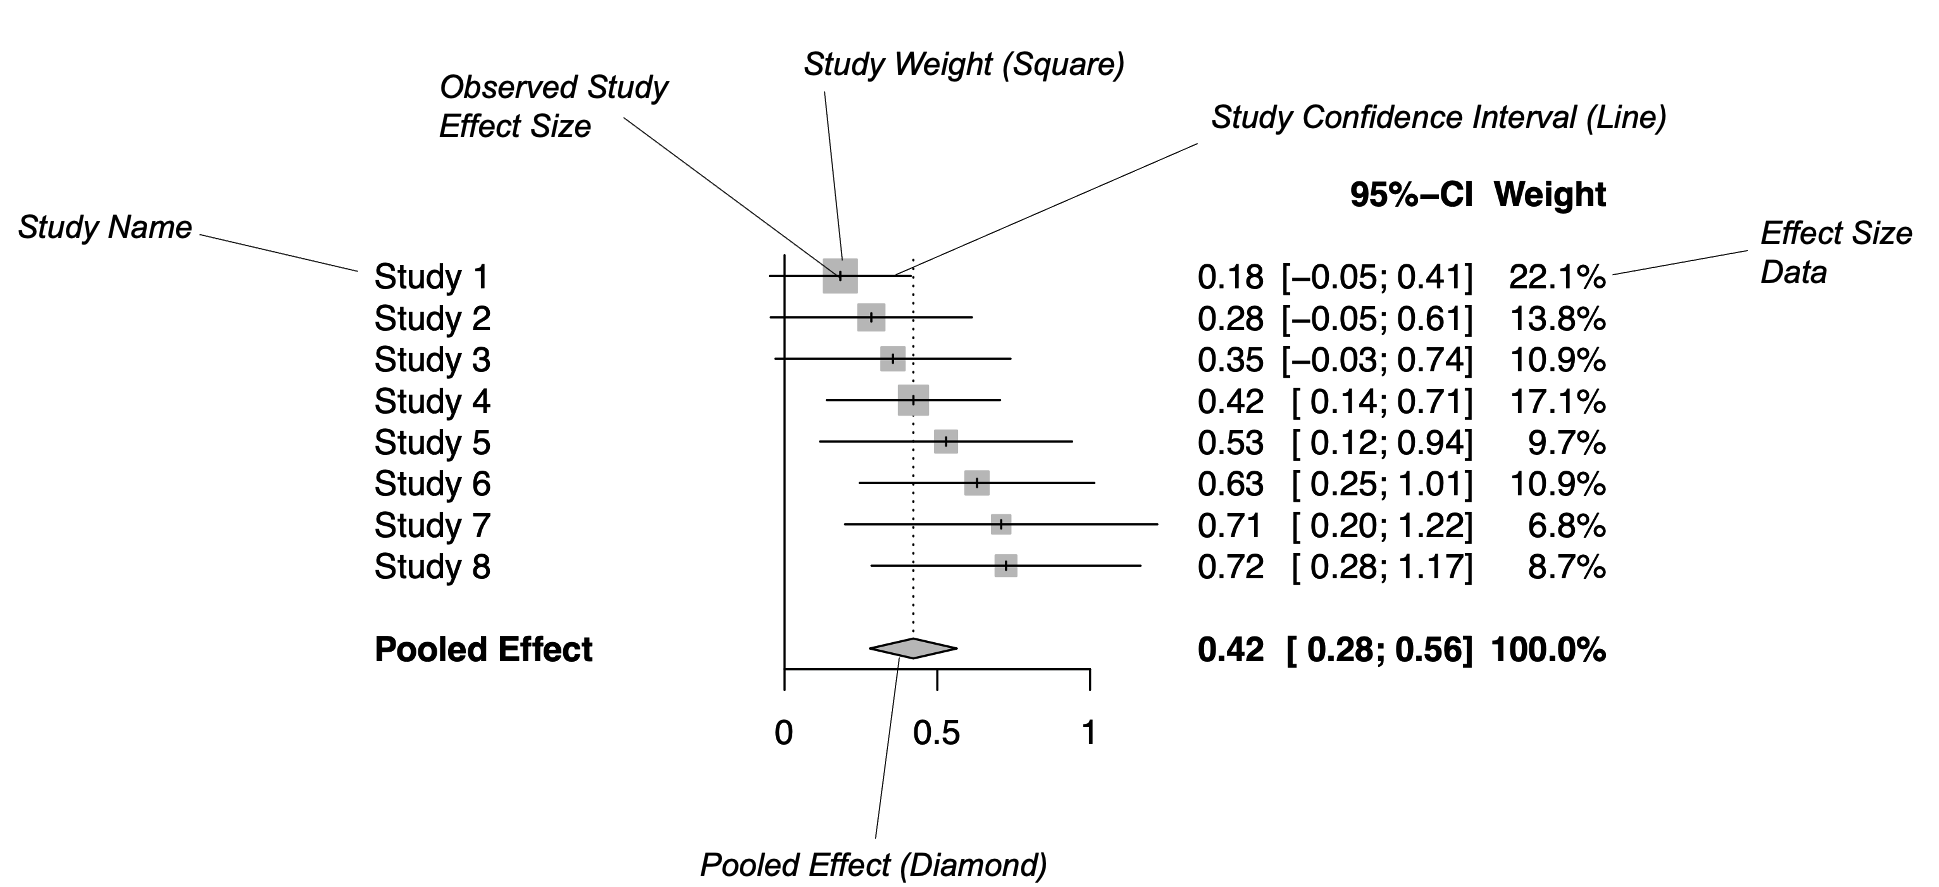
\includegraphics{C:/Users/Admin/Documents/R/WORKING_DIRECTORY/Meta-Analyse\%20Buch/bookdown-demo-master/forest.jpg}
\caption{}
\end{figure}

\begin{rmdinfo}
Now that the created the \textbf{output of our meta-analysis} using the
\texttt{metagen}, \texttt{metacont} or \texttt{metabin} functions in
\texttt{meta} (see \protect\hyperlink{fixed}{Chapter
4.1},\protect\hyperlink{random}{Chapter 4.2} and
\protect\hyperlink{binary}{Chapter 4.3}), it is time to present the data
in a more digestable way.

\textbf{Forest Plots} are an easy way to do this, and it is conventional
to report forest plots in meta-analysis publications.
\end{rmdinfo}

\section{Generating a Forest Plot}\label{generating-a-forest-plot}

To produce a forest plot, we use the meta-analysis output we just
created (e.g., \texttt{m}, \texttt{m.raw}) und the
\texttt{meta::forest()} function. I'll my \texttt{m.hksj.raw} output
from \protect\hyperlink{random.raw}{Chapter 4.2.3} to create the forest
plot

\begin{Shaded}
\begin{Highlighting}[]
\KeywordTok{forest}\NormalTok{(m.hksj.raw)}
\end{Highlighting}
\end{Shaded}

\begin{center}\includegraphics{Doing_Meta_Analysis_in_R_files/figure-latex/unnamed-chunk-73-1} \end{center}

Looks good so far. We see that the function plottet a forest plot with a
\textbf{diamond} (i.e.~the overall effect and its confidence interval)
and a \textbf{prediction interval}.

There are plenty of \textbf{other parameters} within the
\texttt{meta::forest} function which we can use to modify the forest
plot.

\begin{tabular}{l|l|l}
\hline
Type & Parameter & Description\\
\hline
General & sortvar & A sorting variable. For example, you can sort the forest plot by effect size using 'TE', or by author name using 'Author'\\
\hline
General & studlab & This tells the function which variable should be printed as the study label. The standard is 'Author'\\
\hline
General & comb.fixed & Whether fixed effect estimate should be plotted. (TRUE/FALSE)\\
\hline
General & comb.random & Whether random effects estimate should be plotted. (TRUE/FALSE)\\
\hline
General & overall & Whether overall summaries should be plotted. This argument is useful in a meta-analysis with subgroups if summaries should only be plotted on group level.\\
\hline
General & text.fixed & A character string used in the plot to label the pooled fixed effect estimate. Has to be put in "" (e.g. "Overall effect")\\
\hline
General & text.random & A character string used in the plot to label the pooled random effect estimate. Has to be put in "" (e.g. "Overall effect")\\
\hline
General & col.fixed & Line colour (pooled fixed effect estimate). E.g. "red", "blue", or hex color code ("\#2e8aff")\\
\hline
General & col.random & Line colour (random fixed effect estimate). E.g. "red", "blue", or hex color code ("\#2e8aff")\\
\hline
General & prediction & Whether a prediction interval should be printed.\\
\hline
General & text.predict & A character string used in the plot to label the prediction interval. E.g. "Prediction Interval"\\
\hline
General & subgroup & A logical indicating whether subgroup results should be shown in forest plot. This argument is useful in a meta-analysis with subgroups if summaries should not be plotted on group level. (TRUE/FALSE)\\
\hline
General & print.subgroup.labels & A logical indicating whether subgroup label should be printed. (TRUE/FALSE)\\
\hline
General & study.results & Whether results for individual studies should be shown in the figure (useful to only plot subgroup results). (TRUE/FALSE)\\
\hline
General & xlab & A label for the x-axis on the bottom. Put in "".\\
\hline
General & smlab & A label for the summary measure on top. Put in "".\\
\hline
General & xlim & The x limits (min,max) of the plot, or the character "s" to produce symmetric forest plots. This is particularly revelant when your results deviate substantially from zero, or if you also want to have outliers depicted. (e.g. xlim=c(0,1.5) for effects from 0 to 1.5).\\
\hline
General & ref & The reference value to be plotted as a line in the forest plot. This is interesting if you want to compare effects to common thresholds or results from previous analyses (e.g. ref=0.5)\\
\hline
General & leftcols & Here you can specify all variables which should be printed on the left side of your plot. The variables have to be part of you meta-analysis output, so check with name\_of\_your\_output\$ which variables can be displayed. E.g. leftcols=c("TE","seTE").\\
\hline
General & rightcols & Same as leftcols, but for the right side of your plot\\
\hline
General & leftlabs & This specifies how the columns on the left side should be named. Always provide all labels (e.g. leftlabs=c("Author","Effect size","Standard error"))\\
\hline
General & rightlabs & Same as leftlabs, but for the left side of you plot\\
\hline
General & print.I2 & Whether to print the value of the I-squared statistic.\\
\hline
General & print.I2.ci & Whether to print the confidence interval of the I-squared statistic.\\
\hline
General & squaresize & A numeric used to increase or decrease the size of squares in the forest plot. (E.g., squaresize = 1.2)\\
\hline
Color & col.study & The colour for individual study results and confidence limits. E.g. 'red', 'blue', or hex color code ('\#2e8aff')\\
\hline
Color & col.inside & The colour for individual study results and confidence limits if confidence limits are completely within squares. E.g. 'red', 'blue', or hex color code ('\#2e8aff')\\
\hline
Color & col.square & The colour for squares reflecting study's weight in the meta-analysis. E.g. 'red', 'blue', or hex color code ('\#2e8aff')\\
\hline
Color & col.square.lines & The colour for the outer lines of squares reflecting study's weight in the meta-analysis. E.g. 'red', 'blue', or hex color code ('\#2e8aff')\\
\hline
Color & col.diamond & The colour of diamonds representing the results for fixed effect and random effects models. E.g. 'red', 'blue', or hex color code ('\#2e8aff')\\
\hline
Color & col.diamond.fixed & The colour of diamonds for fixed effect estimates. E.g. 'red', 'blue', or hex color code ('\#2e8aff')\\
\hline
Color & col.diamond.random & The colour of diamonds for random effects estimates. E.g. 'red', 'blue', or hex color code ('\#2e8aff')\\
\hline
Color & col.diamond.lines & The colour of the outer lines of diamonds representing the results for fixed effect and random effects models. E.g. 'red', 'blue', or hex color code ('\#2e8aff')\\
\hline
Color & col.diamond.lines.fixed & The colour of the outer lines of diamond for fixed effect estimate. E.g. 'red', 'blue', or hex color code ('\#2e8aff')\\
\hline
Color & col.diamond.lines.random & The colour of the outer lines of diamond for random effects estimate. E.g. 'red', 'blue', or hex color code ('\#2e8aff')\\
\hline
Color & col.inside.fixed & The colour for result of fixed effect meta-analysis if confidence limit lies completely within square. E.g. 'red', 'blue', or hex color code ('\#2e8aff')\\
\hline
Color & col.inside.random & The colour for result of random effects meta-analysis if confidence limit lies completely within square. E.g. 'red', 'blue', or hex color code ('\#2e8aff')\\
\hline
Color & col.predict & Background colour of prediction interval. E.g. 'red', 'blue', or hex color code ('\#2e8aff')\\
\hline
Color & col.predict.lines & Colour of outer lines of prediction interval. E.g. 'red', 'blue', or hex color code ('\#2e8aff')\\
\hline
Color & col.label.right & The colour for label on right side of null effect. E.g. 'red', 'blue', or hex color code ('\#2e8aff')\\
\hline
Color & col.label.left & The colour for label on left side of null effect. E.g. 'red', 'blue', or hex color code ('\#2e8aff')\\
\hline
Digits & digits & Minimal number of significant digits for treatment effects (TE)\\
\hline
Digits & digits.se & Minimal number of significant digits for standard errors\\
\hline
Digits & digits.zval & Minimal number of significant digits for z- or t-statistic for test of overall effect\\
\hline
Digits & digits.tau2 & Minimal number of significant digits for between-study variance\\
\hline
Digits & digits.pval & Minimal number of significant digits for p-value of overall treatment effect\\
\hline
Digits & digits.pval.Q & Minimal number of significant digits for p-value of heterogeneity test\\
\hline
Digits & digits.Q & Minimal number of significant digits for heterogeneity statistic Q\\
\hline
Digits & digits.I2 & Minimal number of significant digits for I-squared statistic\\
\hline
Digits & digits.weight & Minimal number of significant digits for weights\\
\hline
Digits & digits.mean & Minimal number of significant digits for the mean\\
\hline
Digits & digits.sd & Minimal number of significant digits for the standard deviations\\
\hline
\end{tabular}

This is again just an overview. For all settings, type
\texttt{?meta::forest} in your \textbf{console} to see more.

Let's play around with the function a little now:

\begin{Shaded}
\begin{Highlighting}[]
\KeywordTok{forest}\NormalTok{(m.hksj.raw,}
       \DataTypeTok{sortvar=}\NormalTok{TE,}
       \DataTypeTok{xlim =} \KeywordTok{c}\NormalTok{(}\OperatorTok{-}\FloatTok{1.5}\NormalTok{,}\FloatTok{0.5}\NormalTok{),}
       \DataTypeTok{rightlabs =} \KeywordTok{c}\NormalTok{(}\StringTok{"g"}\NormalTok{,}\StringTok{"95% CI"}\NormalTok{,}\StringTok{"weight"}\NormalTok{),}
       \DataTypeTok{leftlabs =} \KeywordTok{c}\NormalTok{(}\StringTok{"Author"}\NormalTok{, }\StringTok{"N"}\NormalTok{,}\StringTok{"Mean"}\NormalTok{,}\StringTok{"SD"}\NormalTok{,}\StringTok{"N"}\NormalTok{,}\StringTok{"Mean"}\NormalTok{,}\StringTok{"SD"}\NormalTok{),}
       \DataTypeTok{lab.e =} \StringTok{"Intervention"}\NormalTok{,}
       \DataTypeTok{pooled.totals =} \OtherTok{FALSE}\NormalTok{,}
       \DataTypeTok{smlab =} \StringTok{""}\NormalTok{,}
       \DataTypeTok{text.random =} \StringTok{"Overall effect"}\NormalTok{,}
       \DataTypeTok{print.tau2 =} \OtherTok{FALSE}\NormalTok{,}
       \DataTypeTok{col.diamond =} \StringTok{"blue"}\NormalTok{,}
       \DataTypeTok{col.diamond.lines =} \StringTok{"black"}\NormalTok{,}
       \DataTypeTok{col.predict =} \StringTok{"black"}\NormalTok{,}
       \DataTypeTok{print.I2.ci =} \OtherTok{TRUE}\NormalTok{,}
       \DataTypeTok{digits.sd =} \DecValTok{2}
\NormalTok{)}
\end{Highlighting}
\end{Shaded}

\begin{center}\includegraphics{Doing_Meta_Analysis_in_R_files/figure-latex/unnamed-chunk-75-1} \end{center}

Looks good so far! For special \textbf{layout types}, proceed to
\protect\hyperlink{layouttypes}{Chapter 5.2} now.

\hypertarget{layouttypes}{\section{Layout types}\label{layouttypes}}

The \texttt{meta::forest} function also has two \textbf{Layouts}
preinstalled which we can use. Those layouts can be accessed with the
\texttt{layout=} parameter.

\begin{itemize}
\tightlist
\item
  \textbf{``RevMan5''}. This layout is used for Cochrane reviews and
  generated by \emph{Review Manager 5}
\item
  \textbf{``JAMA''}. This layout gives you a forest plot according to
  the guidelines of the \emph{Journal of the American Medical
  Association} as output (see details
  \href{https://jamanetwork.com/journals/jama/pages/instructions-for-authors}{here}).
\end{itemize}

The \textbf{RevMan} layout looks like this:

\begin{Shaded}
\begin{Highlighting}[]
\KeywordTok{forest}\NormalTok{(m.hksj.raw,}
       \DataTypeTok{layout =} \StringTok{"RevMan5"}\NormalTok{,}
       \DataTypeTok{digits.sd =} \DecValTok{2}\NormalTok{)}
\end{Highlighting}
\end{Shaded}

\begin{center}\includegraphics{Doing_Meta_Analysis_in_R_files/figure-latex/unnamed-chunk-76-1} \end{center}

The \textbf{JAMA} layout looks like this:

\begin{Shaded}
\begin{Highlighting}[]
\KeywordTok{forest}\NormalTok{(m.hksj.raw,}
       \DataTypeTok{layout =} \StringTok{"JAMA"}\NormalTok{,}
       \DataTypeTok{text.predict =} \StringTok{"95% PI"}\NormalTok{,}
       \DataTypeTok{col.predict =} \StringTok{"black"}\NormalTok{,}
       \DataTypeTok{colgap.forest.left =} \KeywordTok{unit}\NormalTok{(}\DecValTok{15}\NormalTok{,}\StringTok{"mm"}\NormalTok{))}
\end{Highlighting}
\end{Shaded}

\begin{center}\includegraphics{Doing_Meta_Analysis_in_R_files/figure-latex/unnamed-chunk-77-1} \end{center}

\section{Saving the forest plots}\label{saving-the-forest-plots}

Let's say i want to save the JAMA version of my Forest Plot now. To do
this, i have to reuse the code with which i plotted my forest plot, and
put it between
\texttt{pdf(file=\textquotesingle{}name\_of\_the\_pdf\_i\_want\_to\_create.pdf\textquotesingle{})}
and \texttt{dev.off}, both in separate lines. This saves the plot into a
PDF in my Working Directory.

This way, i can export the plot in different formats (you can find more
details on the saving options \protect\hyperlink{saving}{here}).

\textbf{PDF}

\begin{Shaded}
\begin{Highlighting}[]
\KeywordTok{pdf}\NormalTok{(}\DataTypeTok{file=}\StringTok{'forestplot.pdf'}\NormalTok{) }
\NormalTok{forest.jama<-}\KeywordTok{forest}\NormalTok{(m.hksj.raw,}
       \DataTypeTok{layout =} \StringTok{"JAMA"}\NormalTok{,}
       \DataTypeTok{text.predict =} \StringTok{"95% PI"}\NormalTok{,}
       \DataTypeTok{col.predict =} \StringTok{"black"}\NormalTok{,}
       \DataTypeTok{colgap.forest.left =} \KeywordTok{unit}\NormalTok{(}\DecValTok{15}\NormalTok{,}\StringTok{"mm"}\NormalTok{))}
\KeywordTok{dev.off}\NormalTok{() }
\end{Highlighting}
\end{Shaded}

\textbf{PNG}

\begin{Shaded}
\begin{Highlighting}[]
\KeywordTok{png}\NormalTok{(}\DataTypeTok{file=}\StringTok{'forestplot.png'}\NormalTok{) }
\NormalTok{forest.jama<-}\KeywordTok{forest}\NormalTok{(m.hksj.raw,}
       \DataTypeTok{layout =} \StringTok{"JAMA"}\NormalTok{,}
       \DataTypeTok{text.predict =} \StringTok{"95% PI"}\NormalTok{,}
       \DataTypeTok{col.predict =} \StringTok{"black"}\NormalTok{,}
       \DataTypeTok{colgap.forest.left =} \KeywordTok{unit}\NormalTok{(}\DecValTok{15}\NormalTok{,}\StringTok{"mm"}\NormalTok{))}
\KeywordTok{dev.off}\NormalTok{() }
\end{Highlighting}
\end{Shaded}

\textbf{Scalable Vector Graphic}

\begin{Shaded}
\begin{Highlighting}[]
\KeywordTok{svg}\NormalTok{(}\DataTypeTok{file=}\StringTok{'forestplot.svg'}\NormalTok{) }
\NormalTok{forest.jama<-}\KeywordTok{forest}\NormalTok{(m.hksj.raw,}
       \DataTypeTok{layout =} \StringTok{"JAMA"}\NormalTok{,}
       \DataTypeTok{text.predict =} \StringTok{"95% PI"}\NormalTok{,}
       \DataTypeTok{col.predict =} \StringTok{"black"}\NormalTok{,}
       \DataTypeTok{colgap.forest.left =} \KeywordTok{unit}\NormalTok{(}\DecValTok{15}\NormalTok{,}\StringTok{"mm"}\NormalTok{))}
\KeywordTok{dev.off}\NormalTok{() }
\end{Highlighting}
\end{Shaded}

\chapter{Between-study Heterogeneity}\label{between-study-heterogeneity}

\begin{figure}
\centering
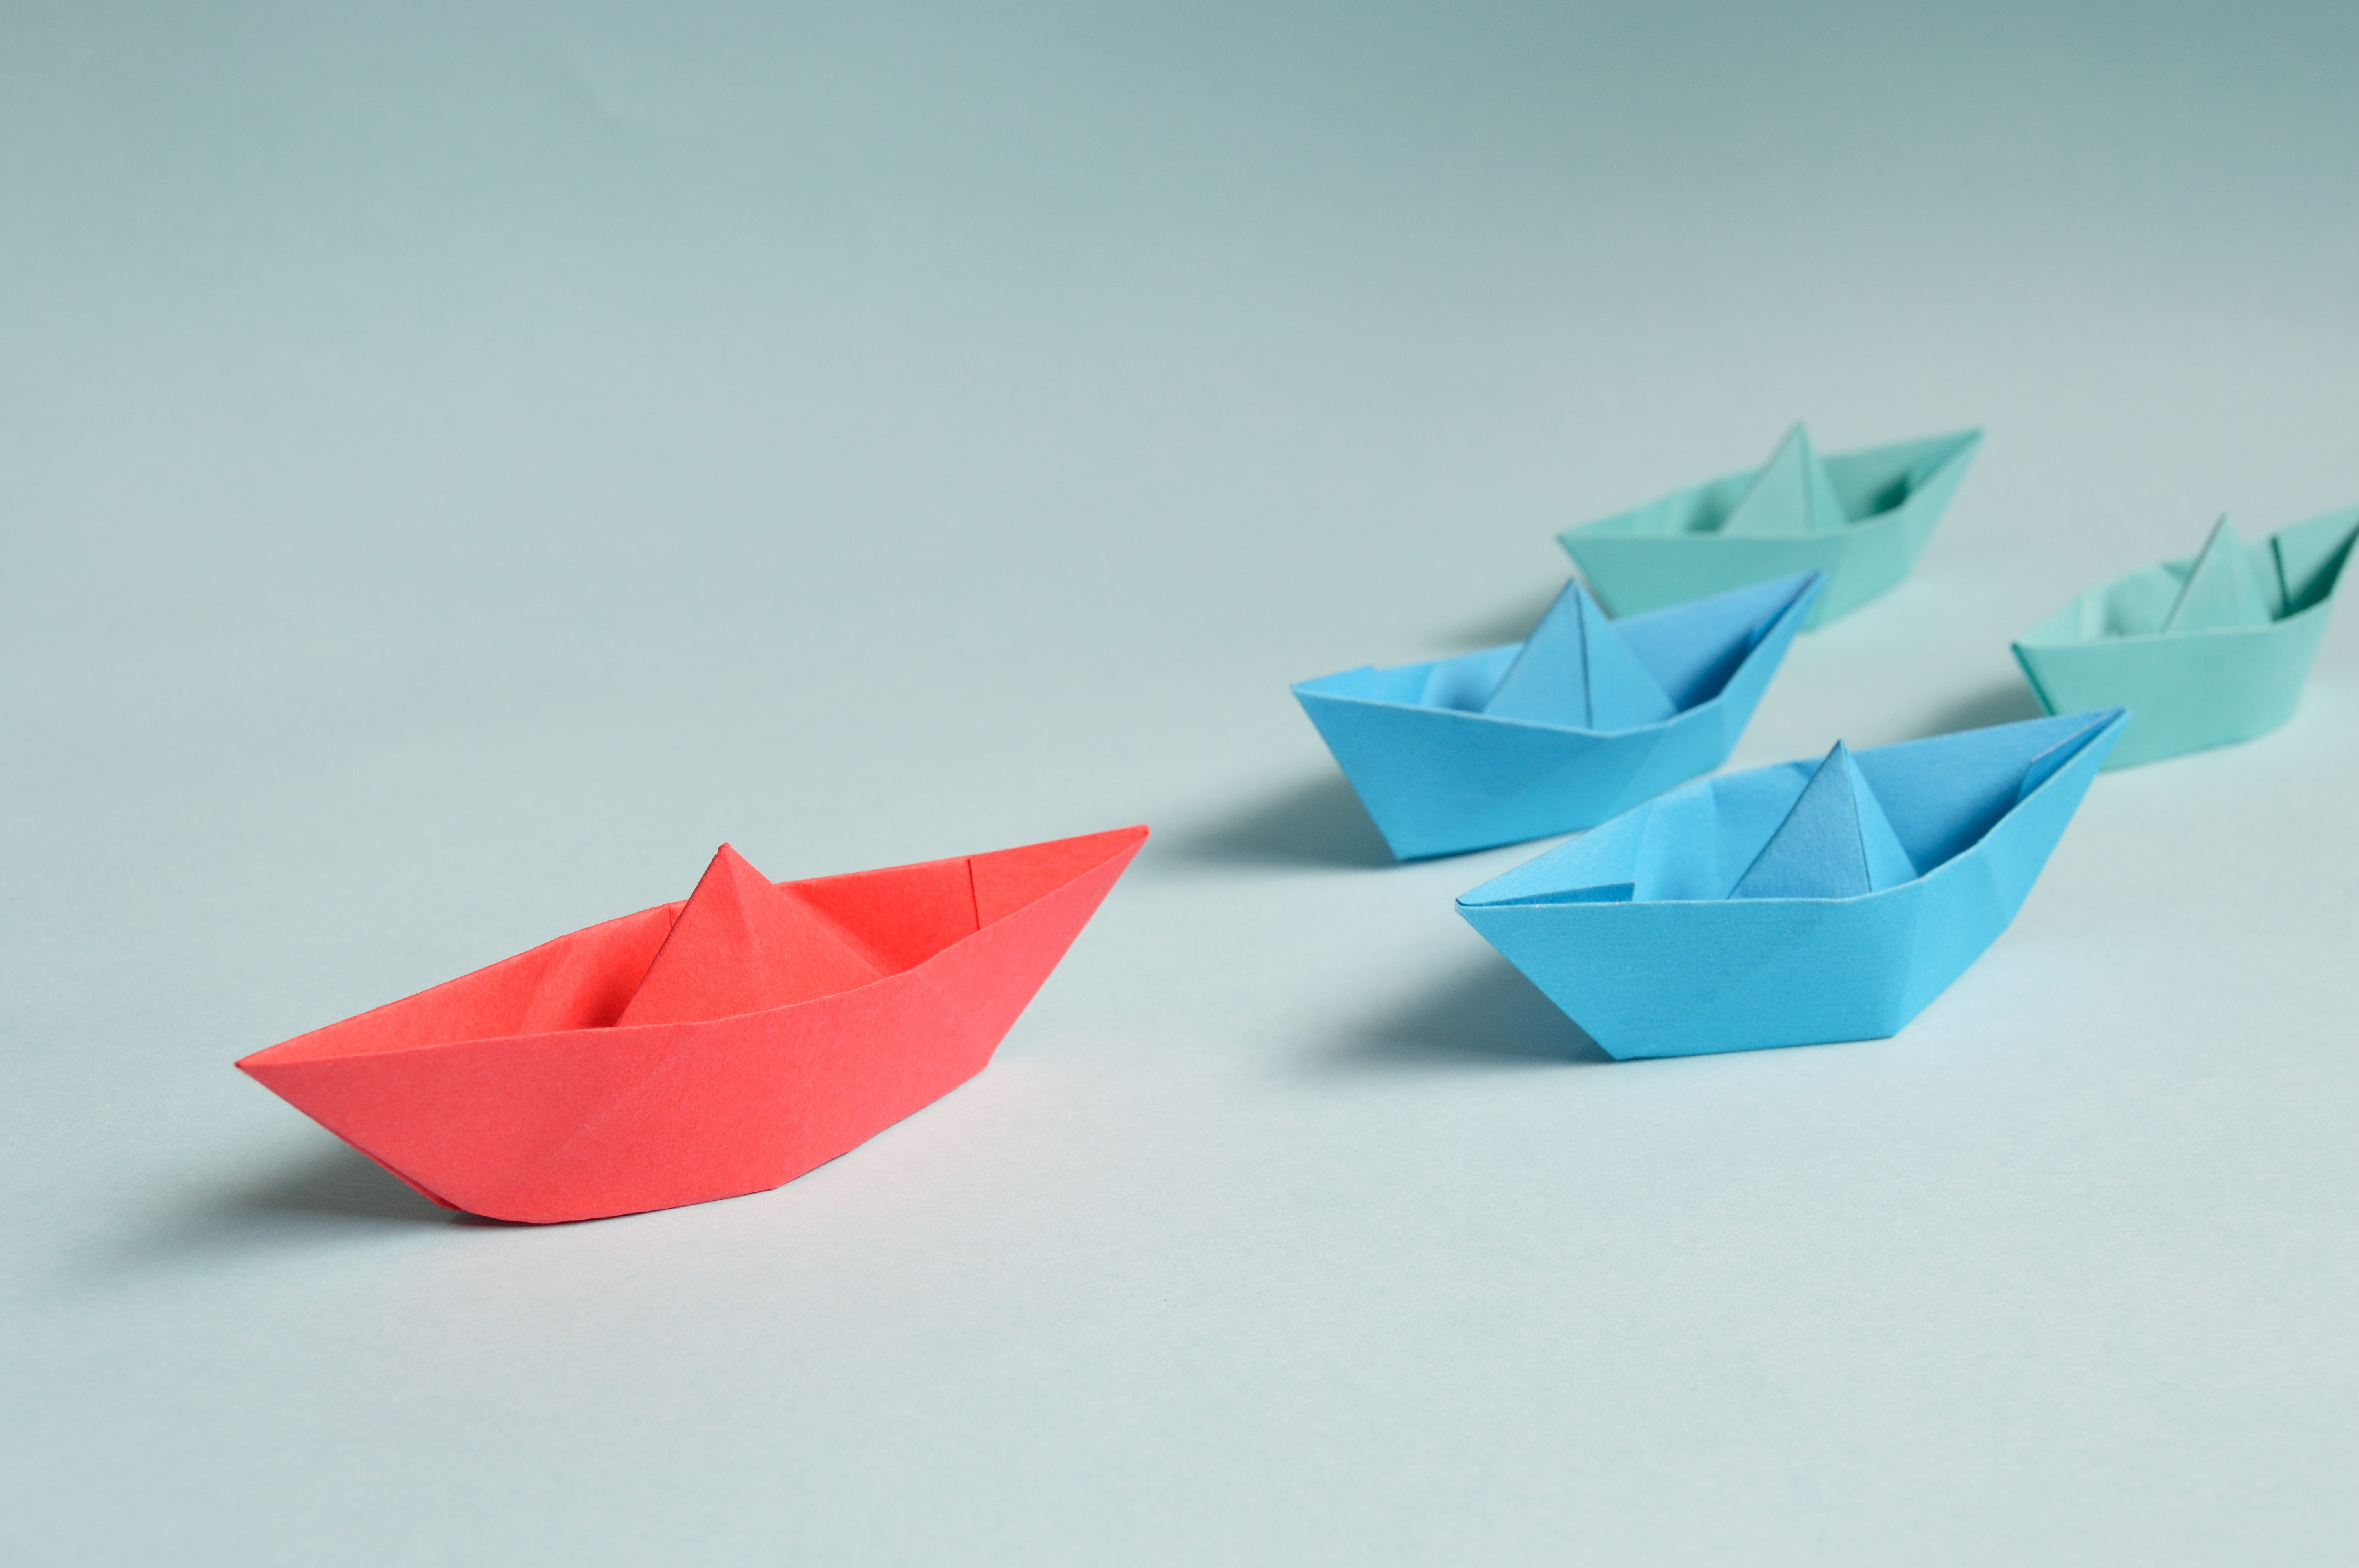
\includegraphics{C:/Users/Admin/Documents/R/WORKING_DIRECTORY/Meta-Analyse\%20Buch/bookdown-demo-master/schiffchen.jpg}
\caption{}
\end{figure}

By now, we have already shown you how to pool effect sizes in a
meta-analysis. In meta-analytic pooling, we aim to \textbf{synthesize
the effects of many different studies into one single effect}. However,
this makes only sense if we aren't comparing \textbf{Apples and
Oranges}. For example, it could be the case that while the overall
effect we calculate in the meta-analysis is \textbf{small}, there are
still a few studies which report \textbf{very high} effect sizes. Such
information is lost in the aggregate effect, but it is very important to
know if all studies, or interventions, yield small effect sizes, or if
there are exceptions.

It could also be the case that even some very \textbf{extreme effect
sizes} were included in the meta-analysis, so-called \textbf{outliers}.
Such outliers might have even distorted our overall effect, and it is
important to how our overall effect would have looked without them.

The extent to which effect sizes vary within a meta-analysis is called
\textbf{heterogeneity}. It is very important to assess heterogeneity in
meta-analyses, as high heterogeneity could be caused by the fact that
there are actually two or more \textbf{subgroups} of studies present in
the data, which have a different true effect. Such information could be
very valuable for \textbf{research}, because this might allow us to find
certain interventions or populations for which effects are lower or
higher.

From a statistical standpoint, high heterogeneity is also problematic.
Very high heterogeneity could mean that the studies have nothing in
common, and that there is no \textbf{``real'' true effect behind our
data}, meaning that it makes no sense to report the pooled effect at all
\citep{borenstein2011}.

\begin{rmdinfo}
\textbf{The idea behind heterogeneity}

Rücker and colleagues {[}@rucker2008undue{]} name three types of
heterogeneity in meta-analyses:

\begin{enumerate}
\def\labelenumi{\arabic{enumi}.}
\tightlist
\item
  \emph{Clinical baseline heterogeneity}. These are differences between
  sample characteristics between the studies. For example, while one
  study might have included rather old people into their study, another
  might have recruited study participants who were mostly quite young.
\item
  \emph{Statistical heterogeneity}. This is the statistical
  heterogeneity we find in our collected effect size data. Such
  heterogeneity migh be either important from a clinical standpoint
  (e.g., when we don't know if a treatment is very or only marginally
  effective because the effects vary much from study to study), or from
  statistical standpoint (because it dilutes the confidence we have in
  our pooled effect)
\item
  \emph{Other sources of heterogeneity}, such as design-related
  heterogeneity.
\end{enumerate}

Point 1. and 3. may be controlled for to some extent by restricting the
scope of our search for studies to certain well-defined intervention
types, populations, and outcomes.

Point 2., on the other hand, has to be assessed once we conducted the
pooling of studies. This is what this chapter focuses on.
\end{rmdinfo}

\begin{rmdinfo}
\textbf{Heterogeneity Measures}

There are \textbf{three types of heterogeneity measures} which are
commonly used to assess the degree of heterogeneity. In the following
examples, \(k\) denotes the individual study, \(K\) denotes all studies
in our meta-analysis, \(\hat \theta_k\) is the estimated effect of \(k\)
with a variance of \(\hat \sigma^{2}_k\), and \(w_k\) is the individual
\textbf{weight} of the study (i.e., its \emph{inverse variance}:
\(w_k = \frac{1}{\hat \sigma^{2}_k}\); see infobox in
\protect\hyperlink{fixed}{Chapter 4.1.1} for more details).

\textbf{1. Cochran's \emph{Q} }

For Cochran's \emph{Q}-statistic, is the \textbf{difference between the
observed effect sizes and the fixed-effect model estimate} of the effect
size, which is then \textbf{squared, weighted and summed}.

\[ Q = \sum\limits_{k=1}^K w_k (\hat\theta_k  - \frac{\sum\limits_{k=1}^K w_k \hat\theta_k}{\sum\limits_{k=1}^K w_k})^{2}\]

\textbf{2. Higgin's \& Thompson's \emph{I}\textsuperscript{2} }

\(I^{2}\) {[}@higgins2002quantifying{]} is the \textbf{percentage of
variability} in the effect size estimates which is not caused by
sampling error. It is derived from \(Q\):

\[I^{2} = max \left\{0, \frac{Q-(K-1)}{Q}  \right\}\]

\textbf{3. Tau-squared}

\(\tau^{2}\) is the between-study variance in our meta-analysis. As we
show in \protect\hyperlink{tau2}{Chapter 4.2.1}, there are various
proposed ways to calculate \(\tau^{2}\)
\end{rmdinfo}

\begin{rmdachtung}
\textbf{Which measure should i use?}

Generally, when we assess and report heterogeneity in a meta-analysis,
we need a measure which is \textbf{robust, and not to easily influenced
by statistical power}.

\textbf{Cochrane's \emph{Q} } increases both when the \textbf{number of
studies} (\(k\)) increases, and when the \textbf{precision} (i.e., the
sample size \(N\) of a study) increases. Therefore, \emph{Q} and weather
it is \textbf{significant} highly depends on the size of your
meta-analysis, and thus its statistical power. We should therefore not
only rely on \emph{Q} when assessing heterogeneity.

\textbf{I\textsuperscript{2}} on the other hand, is not sensitive to
changes in the number of studies in the analyses. I\textsuperscript{2}
is therefore used extensively in medical and psychological research,
especially since there is a \textbf{``rule of thumb''} to interpret it
{[}@higgins2003measuring{]}:

\begin{itemize}
\tightlist
\item
  I\textsuperscript{2} = 25\%: \textbf{low heterogeneity}
\item
  I\textsuperscript{2} = 50\%: \textbf{moderate heterogeneity}
\item
  I\textsuperscript{2} = 75\%: \textbf{substantial heterogeneity}
\end{itemize}

Despite its common use in the literature, I\textsuperscript{2} not
always an adequate measure for heterogeneity either, because it still
heavily depends on the \textbf{precision} of the included studies
{[}@rucker2008undue; @borenstein2017basics{]}. As said before, \(I^{2}\)
is simply the amount of variability \textbf{not caused by sampling
error}. If our studies become increasingly large, this sampling error
tends to \textbf{zero}, while at the same time, \(I^{2}\) tends to 100\%
simply because the single studies have greater \(N\). Only relying on
I\textsuperscript{2} is therefore not a good option either.

\textbf{Tau-squared}, on the other hand, is \textbf{insensitive} to the
number of studies, \textbf{and} the precision. Yet, it is often hard to
interpret how relevant our tau-squared is from a practicial standpoint.

\textbf{Prediction intervals} (like the ones we automatically calculated
in \protect\hyperlink{pool}{Chapter 4}) are a good way to overcome this
limitation {[}@inthout2016plea{]}, as they take our between-study
variance into account. Prediction intervals give us a range for which we
can \textbf{expect the effects of future studies to fall} based on
\textbf{our present evidence in the meta-analysis}. If our prediction
interval, for example, lies completely on the positive side favoring the
intervention, we can be quite confident to say that \textbf{despite
varying effects, the intervention might be at least in some way
beneficial in all contexts we studied in the future}. If the confidence
interval includes \textbf{zero}, we can be less sure about this,
although it should be noted that \textbf{broad prediction intervals are
quite common, especially in medicine and psychology}.
\end{rmdachtung}

\section{Define analyzed meta-analysis
output}\label{define-analyzed-meta-analysis-output}

\begin{Shaded}
\begin{Highlighting}[]
\NormalTok{influence.data<-m.hksj}
\end{Highlighting}
\end{Shaded}

\begin{Shaded}
\begin{Highlighting}[]
\NormalTok{res <-}\StringTok{ }\KeywordTok{rma}\NormalTok{(}\DataTypeTok{yi=}\NormalTok{TE, }\DataTypeTok{sei=}\NormalTok{seTE, }\DataTypeTok{measure=}\StringTok{"ZCOR"}\NormalTok{, }
           \DataTypeTok{data=}\NormalTok{influence.data, }
           \DataTypeTok{method =} \StringTok{"SJ"}\NormalTok{, }
           \DataTypeTok{test=}\StringTok{"knha"}\NormalTok{)}
\NormalTok{inf <-}\StringTok{ }\KeywordTok{influence}\NormalTok{(res)}
\NormalTok{influence.data.metainf<-}\KeywordTok{metainf}\NormalTok{(influence.data)}
\NormalTok{influence.data.metainf}\OperatorTok{$}\NormalTok{I2<-}\KeywordTok{format}\NormalTok{(}\KeywordTok{round}\NormalTok{(influence.data.metainf}\OperatorTok{$}\NormalTok{I2,}\DecValTok{2}\NormalTok{),}\DataTypeTok{nsmall=}\DecValTok{2}\NormalTok{)}
\KeywordTok{plot}\NormalTok{(inf)}
\KeywordTok{baujat}\NormalTok{(influence.data)}
\KeywordTok{forest}\NormalTok{(influence.data.metainf,}
       \DataTypeTok{sortvar=}\NormalTok{I2,}
       \DataTypeTok{rightcols =} \KeywordTok{c}\NormalTok{(}\StringTok{"TE"}\NormalTok{,}\StringTok{"ci"}\NormalTok{,}\StringTok{"I2"}\NormalTok{),}
       \DataTypeTok{smlab =} \StringTok{"Sorted by I-squared"}\NormalTok{)}
\KeywordTok{forest}\NormalTok{(influence.data.metainf,}
       \DataTypeTok{sortvar=}\NormalTok{TE,}
       \DataTypeTok{rightcols =} \KeywordTok{c}\NormalTok{(}\StringTok{"TE"}\NormalTok{,}\StringTok{"ci"}\NormalTok{,}\StringTok{"I2"}\NormalTok{),}
       \DataTypeTok{smlab =} \StringTok{"Sorted by Effect size"}\NormalTok{)}
\end{Highlighting}
\end{Shaded}

\begin{figure}

{\centering \includegraphics{Doing_Meta_Analysis_in_R_files/figure-latex/unnamed-chunk-88-1} 

}

\caption{Influence Analyses}\label{fig:unnamed-chunk-88}
\end{figure}\begin{figure}

{\centering \includegraphics{Doing_Meta_Analysis_in_R_files/figure-latex/unnamed-chunk-89-1} 

}

\caption{Baujat Plot}\label{fig:unnamed-chunk-89}
\end{figure}

\begin{figure}

{\centering \includegraphics{Doing_Meta_Analysis_in_R_files/figure-latex/unnamed-chunk-90-1} 

}

\caption{Leave-One-Out-Analyses}\label{fig:unnamed-chunk-901}
\end{figure}\begin{figure}

{\centering \includegraphics{Doing_Meta_Analysis_in_R_files/figure-latex/unnamed-chunk-90-2} 

}

\caption{Leave-One-Out-Analyses}\label{fig:unnamed-chunk-902}
\end{figure}

\chapter{Creating a RevMan style Risk of Bias
summary}\label{creating-a-revman-style-risk-of-bias-summary}

\begin{figure}
\centering
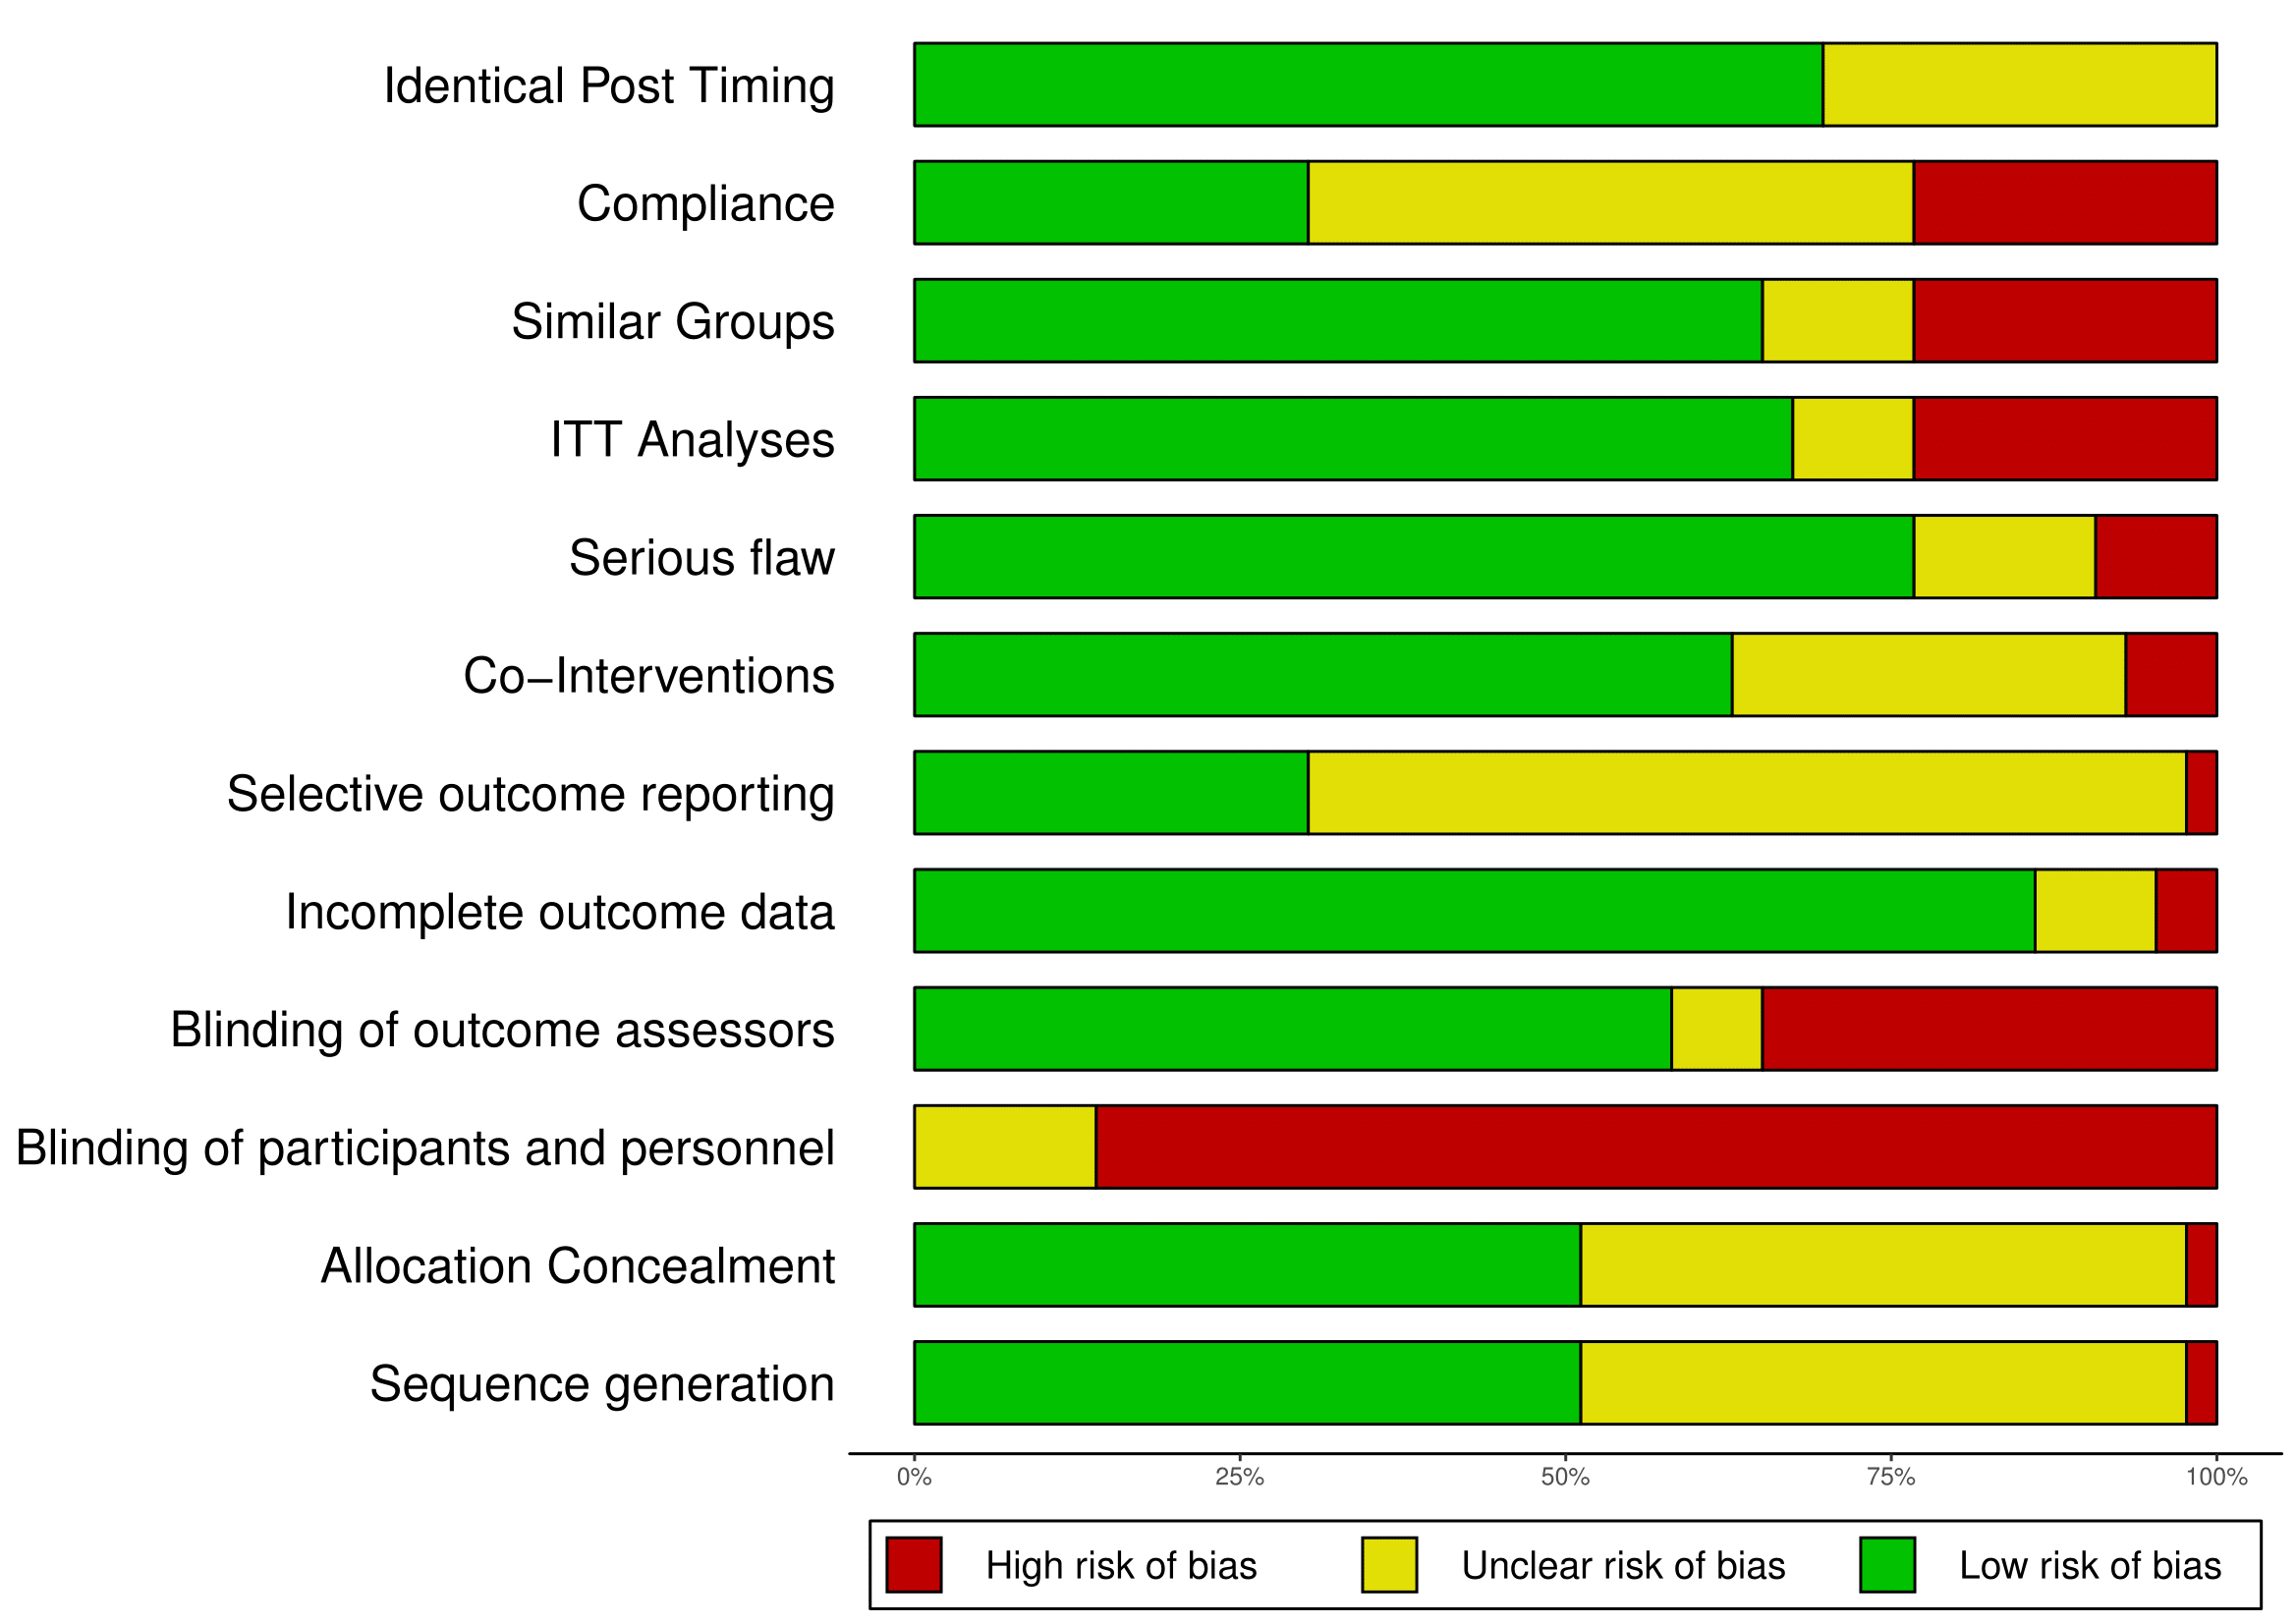
\includegraphics{C:/Users/Admin/Documents/R/WORKING_DIRECTORY/Meta-Analyse\%20Buch/bookdown-demo-master/robplot.PNG}
\caption{A finished Risk of Bias summary}
\end{figure}

\section{Preparing your Risk of Bias
data}\label{preparing-your-risk-of-bias-data}

In many Meta-Analyses, you will also want to have a look at the quality
of included studies using the
\href{https://handbook-5-1.cochrane.org/chapter_8/8_6_presentation_of_assessments_of_risk_of_bias.htm}{\textbf{RevMan
Risk of Bias assessment tool}}. However, many researchers don't use
\textbf{RevMan} to conduct Meta-Analyses, one has to put some extra
effort into inserting all study quality data by hand into RevMan, which
is extremely time-consuming.

Furthermore, the quality of the Risk of Bias (RoB) summary figures in
RevMan are of suboptimal picture quality. Many journals will require
figures with better quality, or figures saved in another format (such as
\textbf{.svg} or \textbf{.pdf}).

\begin{figure}
\centering
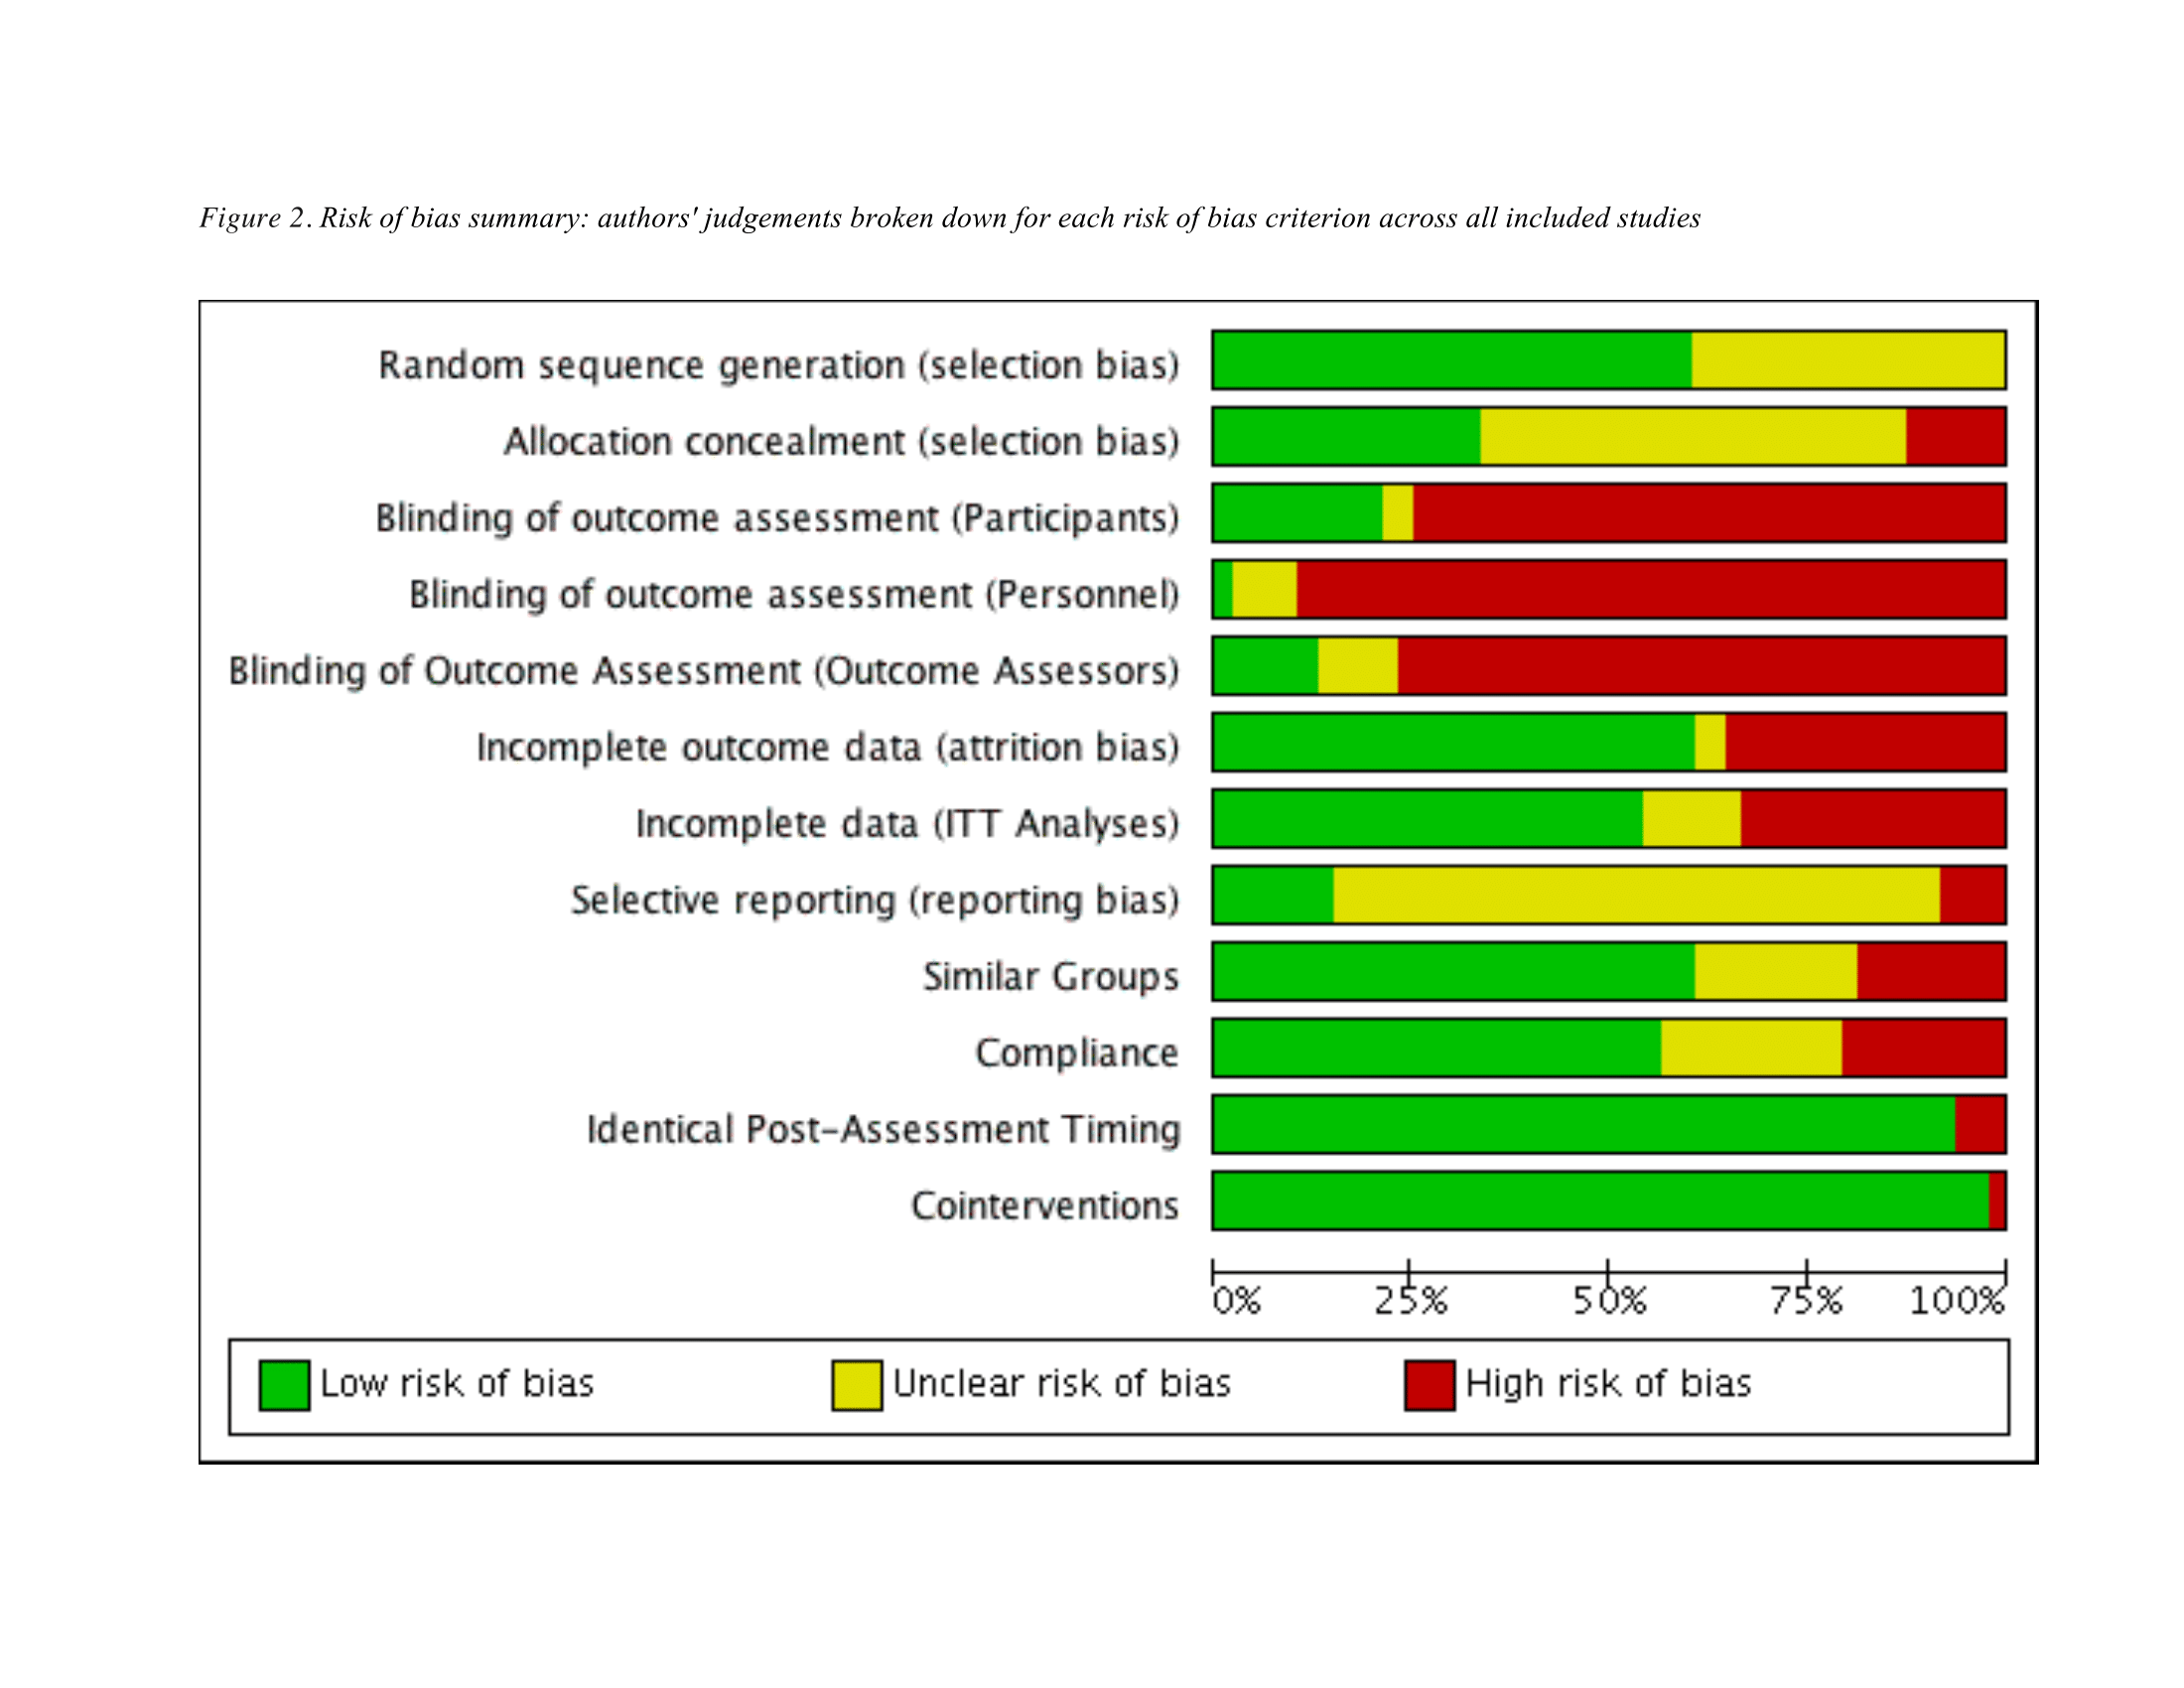
\includegraphics{C:/Users/Admin/Documents/R/WORKING_DIRECTORY/Meta-Analyse\%20Buch/bookdown-demo-master/robsummaryrevman.png}
\caption{This is the output created by RevMan}
\end{figure}

To avoid all of this, you can easily plot the \textbf{RoB Summary in
RStudio yourself}. To do this, we again have to prepare an EXCEL sheet
in which we store our RoB data. In
\protect\hyperlink{excel_preparation}{Chapter 3.1.1}, we already
described how the preparation and import of EXCEL sheets into RStudio
works in general. For this data sheet, you need to follow a few
guidelines:

\begin{itemize}
\tightlist
\item
  Name the first column \textbf{Author}, and put all the study names in
  this column (e.g., Frogeli et al.)
\item
  Give the other \textbf{columns a name signifying the RoB criterion}
  you assessed. Do this for all criteria you want to have included in
  your plot. \textbf{Important}: when naming your column, do not use
  spaces between word, but use underscores or points instead
  (e.g.~allocation\_concealment)
\item
  In these columns, you have to describe if the study received a
  \textbf{High}, \textbf{Low}, or \textbf{Unclear} risk of bias rating.
  Use exactly these codes for your data, including upper and lowercase
  (R is case sensitive)
\item
  Do \textbf{not} store any other information in your data
  (e.g.~commentaries on your RoB decision)
\end{itemize}

\section{Plotting the summary}\label{plotting-the-summary}

To plot the summary, we have to import our dataset first. We describe
how to do this in \protect\hyperlink{import_excel}{Chapter 3.2}. I
simply called my dataset \texttt{rob}.

Let's have a look at the structure of the data first:

\begin{Shaded}
\begin{Highlighting}[]
\KeywordTok{str}\NormalTok{(rob)}
\end{Highlighting}
\end{Shaded}

\begin{verbatim}
## Classes 'tbl_df', 'tbl' and 'data.frame':    43 obs. of  13 variables:
##  $ RoB_sequence                                : chr  "Low" "Low" "Low" "Low" ...
##  $ RoB_allocation_concealment_                 : chr  "Low" "Low" "Low" "Low" ...
##  $ RoB_Blinding of participants and personnel  : chr  "High" "High" "High" "High" ...
##  $ RoB_Blinding of outcome assessors           : chr  "Low" "Low" "Low" "Low" ...
##  $ RoB_Incomplete outcome data for all outcomes: chr  "Low" "Low" "Low" "Low" ...
##  $ RoB_Selective outcome reporting             : chr  "Low" "Unclear" "Low" "Low" ...
##  $ RoB_Co-interventions                        : chr  "Unclear" "Low" "Low" "Low" ...
##  $ RoB_Serious_flaw                            : chr  "Low" "Low" "Low" "Low" ...
##  $ RoB_ITT                                     : chr  "Low" "Low" "Low" "Low" ...
##  $ RoB_SimilarGroups                           : chr  "Unclear" "Low" "Low" "Low" ...
##  $ RoB_compliance                              : chr  "Low" "Unclear" "High" "High" ...
##  $ RoB_identical_post_timing                   : chr  "Low" "Low" "Low" "Low" ...
##  $ Author                                      : chr  "BiesheuvelLeliefeld 2017" "Bockting 2005 & 2010 & 2015" "Bockting 2018" "Bockting 2018" ...
\end{verbatim}

We can see that we have the data imported in RStudio now, with ratings
for every criterion in each column. If you named your columns
differently, or used less or more criteria, this is not that important
now. We will get to this later.

We will plot the summary using the packages \texttt{ggplot2} and
\texttt{tidyr}. They should be installed as part of the
\texttt{tidyverse}, but be sure to have it on your computer, and then
load them from your \textbf{library}.

\begin{Shaded}
\begin{Highlighting}[]
\KeywordTok{library}\NormalTok{(ggplot2)}
\KeywordTok{library}\NormalTok{(tidyr)}
\end{Highlighting}
\end{Shaded}

We can than use a predefined code to generate our first plot. To do
this, we have to check if a few things about our dataset are correctly
defined.

\begin{enumerate}
\def\labelenumi{\arabic{enumi}.}
\tightlist
\item
  You have to rename your dataset to \texttt{rob} for the syntax to
  work. In my case, the dataset already has this name, so it is kind of
  redundant. Paste the name of your dataset on the right side of the
  arrow to rename your data using this code:
\end{enumerate}

\begin{Shaded}
\begin{Highlighting}[]
\NormalTok{rob<-Name.of.your.data}
\end{Highlighting}
\end{Shaded}

\begin{enumerate}
\def\labelenumi{\arabic{enumi}.}
\setcounter{enumi}{1}
\tightlist
\item
  We have to \textbf{transform our data for the plot}. To do this, we
  only have to check in our dataset which risk of bias criterion appears
  first, and which appears last in our file. To do this, we'll use the
  \texttt{str()} function again
\end{enumerate}

\begin{Shaded}
\begin{Highlighting}[]
\KeywordTok{str}\NormalTok{(rob)}
\end{Highlighting}
\end{Shaded}

\begin{verbatim}
## Classes 'tbl_df', 'tbl' and 'data.frame':    43 obs. of  13 variables:
##  $ RoB_sequence                                : chr  "Low" "Low" "Low" "Low" ...
##  $ RoB_allocation_concealment_                 : chr  "Low" "Low" "Low" "Low" ...
##  $ RoB_Blinding of participants and personnel  : chr  "High" "High" "High" "High" ...
##  $ RoB_Blinding of outcome assessors           : chr  "Low" "Low" "Low" "Low" ...
##  $ RoB_Incomplete outcome data for all outcomes: chr  "Low" "Low" "Low" "Low" ...
##  $ RoB_Selective outcome reporting             : chr  "Low" "Unclear" "Low" "Low" ...
##  $ RoB_Co-interventions                        : chr  "Unclear" "Low" "Low" "Low" ...
##  $ RoB_Serious_flaw                            : chr  "Low" "Low" "Low" "Low" ...
##  $ RoB_ITT                                     : chr  "Low" "Low" "Low" "Low" ...
##  $ RoB_SimilarGroups                           : chr  "Unclear" "Low" "Low" "Low" ...
##  $ RoB_compliance                              : chr  "Low" "Unclear" "High" "High" ...
##  $ RoB_identical_post_timing                   : chr  "Low" "Low" "Low" "Low" ...
##  $ Author                                      : chr  "BiesheuvelLeliefeld 2017" "Bockting 2005 & 2010 & 2015" "Bockting 2018" "Bockting 2018" ...
\end{verbatim}

We see that our dataset starts with the variable \texttt{RoB\_sequence},
and that the last RoB column is \texttt{RoB\_identifcal\_post\_timing}.

We now have to tell the transformation function that we want all RoB
criteria, from \texttt{RoB\_sequence} to
\texttt{RoB\_identifcal\_post\_timing}, to be included in the plot. To
do this, we have to insert
\texttt{RoB\_sequence:RoB\_identifcal\_post\_timing} after
\texttt{measurement} in the following code:

\begin{Shaded}
\begin{Highlighting}[]
\NormalTok{rob.long <-}\StringTok{ }\KeywordTok{gather}\NormalTok{(rob, }
\NormalTok{                   condition, measurement, }
\NormalTok{                   RoB_sequence}\OperatorTok{:}\NormalTok{RoB_identical_post_timing, }
                   \DataTypeTok{factor_key=}\OtherTok{TRUE}\NormalTok{)}
\NormalTok{rob.long}\OperatorTok{$}\NormalTok{measurement<-}\KeywordTok{as.factor}\NormalTok{(rob.long}\OperatorTok{$}\NormalTok{measurement)}
\NormalTok{rob.long}\OperatorTok{$}\NormalTok{measurement<-}\KeywordTok{factor}\NormalTok{(rob.long}\OperatorTok{$}\NormalTok{measurement,}
                             \KeywordTok{levels}\NormalTok{(rob.long}\OperatorTok{$}\NormalTok{measurement)[}\KeywordTok{c}\NormalTok{(}\DecValTok{1}\NormalTok{,}\DecValTok{3}\NormalTok{,}\DecValTok{2}\NormalTok{)])}
\end{Highlighting}
\end{Shaded}

The rest of the code, we can leave as is. Note that the string
\texttt{RoB\_sequence:RoB\_identifcal\_post\_timing} can look totally
different for you, because you only have to use the names of the column
that you have for your dataset.

So, if your first RoB column in the dataset was
\texttt{allocation\_concealment}, and your last one
\texttt{cointerventions}, the string would be called
\texttt{allocation\_concealment:cointerventions}, and the code would
look like this:

\begin{Shaded}
\begin{Highlighting}[]
\NormalTok{rob.long <-}\StringTok{ }\KeywordTok{gather}\NormalTok{(rob, }
\NormalTok{                   condition, measurement, }
\NormalTok{                   allocation_concealment}\OperatorTok{:}\NormalTok{cointerventions, }
                   \DataTypeTok{factor_key=}\OtherTok{TRUE}\NormalTok{)}
\NormalTok{rob.long}\OperatorTok{$}\NormalTok{measurement<-}\KeywordTok{as.factor}\NormalTok{(rob.long}\OperatorTok{$}\NormalTok{measurement)}
\NormalTok{rob.long}\OperatorTok{$}\NormalTok{measurement<-}\KeywordTok{factor}\NormalTok{(rob.long}\OperatorTok{$}\NormalTok{measurement,}
                             \KeywordTok{levels}\NormalTok{(rob.long}\OperatorTok{$}\NormalTok{measurement)[}\KeywordTok{c}\NormalTok{(}\DecValTok{1}\NormalTok{,}\DecValTok{3}\NormalTok{,}\DecValTok{2}\NormalTok{)])}
\end{Highlighting}
\end{Shaded}

\begin{enumerate}
\def\labelenumi{\arabic{enumi}.}
\setcounter{enumi}{2}
\tightlist
\item
  Now, it's time to plot our first graph. We will call this plot
  \texttt{rob.summary}. As you've prepared your data already, just run
  the code below:
\end{enumerate}

\begin{Shaded}
\begin{Highlighting}[]
\NormalTok{rob.summary<-}\KeywordTok{ggplot}\NormalTok{(}\DataTypeTok{data=}\NormalTok{rob.long)}\OperatorTok{+}
\StringTok{  }\KeywordTok{geom_bar}\NormalTok{(}\DataTypeTok{mapping=}\KeywordTok{aes}\NormalTok{(}\DataTypeTok{x=}\NormalTok{condition,}\DataTypeTok{fill=}\NormalTok{measurement),}
           \DataTypeTok{width=}\FloatTok{0.7}\NormalTok{, }
           \DataTypeTok{position =} \StringTok{"fill"}\NormalTok{,}
           \DataTypeTok{color=}\StringTok{"black"}\NormalTok{)}\OperatorTok{+}
\StringTok{  }\KeywordTok{coord_flip}\NormalTok{(}\DataTypeTok{ylim =} \KeywordTok{c}\NormalTok{(}\DecValTok{0}\NormalTok{,}\DecValTok{1}\NormalTok{))}\OperatorTok{+}
\StringTok{  }\KeywordTok{guides}\NormalTok{(}\DataTypeTok{fill =} \KeywordTok{guide_legend}\NormalTok{(}\DataTypeTok{reverse =} \OtherTok{TRUE}\NormalTok{))}\OperatorTok{+}
\StringTok{  }\KeywordTok{scale_fill_manual}\NormalTok{(}\StringTok{"Risk of Bias"}\NormalTok{,}
                    \DataTypeTok{labels =} \KeywordTok{c}\NormalTok{(}\StringTok{"    High risk of bias          "}\NormalTok{,}
                               \StringTok{"    Unclear risk of bias       "}\NormalTok{,}
                               \StringTok{"    Low risk of bias  "}\NormalTok{),}
                    \DataTypeTok{values =} \KeywordTok{c}\NormalTok{(}\StringTok{"Unclear"}\NormalTok{ =}\StringTok{ "#E2DF07"}\NormalTok{,}
                               \StringTok{"High"}\NormalTok{ =}\StringTok{ "#BF0000"}\NormalTok{,}
                               \StringTok{"Low"}\NormalTok{ =}\StringTok{ "#02C100"}\NormalTok{))}\OperatorTok{+}
\StringTok{  }\KeywordTok{scale_y_continuous}\NormalTok{(}\DataTypeTok{labels =}\NormalTok{ scales}\OperatorTok{::}\NormalTok{percent)}\OperatorTok{+}
\StringTok{  }\KeywordTok{theme}\NormalTok{(}\DataTypeTok{axis.title.x=}\KeywordTok{element_blank}\NormalTok{(),}
        \DataTypeTok{axis.title.y.left=}\KeywordTok{element_blank}\NormalTok{(),}
        \DataTypeTok{axis.ticks.y=}\KeywordTok{element_blank}\NormalTok{(),}
        \DataTypeTok{axis.text.y.left =} \KeywordTok{element_text}\NormalTok{(}\DataTypeTok{size=}\DecValTok{18}\NormalTok{, }\DataTypeTok{color =} \StringTok{"black"}\NormalTok{),}
        \DataTypeTok{axis.line.x =} \KeywordTok{element_line}\NormalTok{(}\DataTypeTok{colour =} \StringTok{"black"}\NormalTok{, }
                                 \DataTypeTok{size =} \FloatTok{0.5}\NormalTok{, }\DataTypeTok{linetype =} \StringTok{"solid"}\NormalTok{),}
        \DataTypeTok{legend.position =} \StringTok{"bottom"}\NormalTok{,}
        \DataTypeTok{panel.grid.major =} \KeywordTok{element_blank}\NormalTok{(), }
        \DataTypeTok{panel.grid.minor =} \KeywordTok{element_blank}\NormalTok{(),}
        \DataTypeTok{panel.background =} \KeywordTok{element_blank}\NormalTok{(),}
        \DataTypeTok{legend.background =} \KeywordTok{element_rect}\NormalTok{(}\DataTypeTok{linetype=}\StringTok{"solid"}\NormalTok{, }
                                         \DataTypeTok{colour =}\StringTok{"black"}\NormalTok{),}
        \DataTypeTok{legend.title =} \KeywordTok{element_blank}\NormalTok{(),}
        \DataTypeTok{legend.key.size =} \KeywordTok{unit}\NormalTok{(}\FloatTok{0.75}\NormalTok{,}\StringTok{"cm"}\NormalTok{),}
        \DataTypeTok{legend.text=}\KeywordTok{element_text}\NormalTok{(}\DataTypeTok{size=}\DecValTok{14}\NormalTok{))}
\NormalTok{rob.summary}
\end{Highlighting}
\end{Shaded}

\includegraphics{Doing_Meta_Analysis_in_R_files/figure-latex/unnamed-chunk-98-1.pdf}

\begin{enumerate}
\def\labelenumi{\arabic{enumi}.}
\setcounter{enumi}{3}
\item
  We see that RStudio has already \textbf{created a RoB summary plot},
  but there's something missing. The labels for each RoB criterion on
  the left are the \textbf{raw names} we gave each column, so we should
  change them to their actual name. To do this, we have to attach the
  correct labels for each criterion to our \texttt{rob.summary}plot.
\item
  To do this, we have to attach \texttt{+} a function which describes
  which label should be replaced with which name. A generic version
  looks like this:
\end{enumerate}

\begin{Shaded}
\begin{Highlighting}[]
\NormalTok{rob.summary<-rob.summary}\OperatorTok{+}
\StringTok{  }\KeywordTok{scale_x_discrete}\NormalTok{(}\DataTypeTok{labels=}\KeywordTok{c}\NormalTok{(}\StringTok{"former_criterion_name_1"}\NormalTok{ =}\StringTok{ "New Criterion Name 1"}\NormalTok{, }
                            \StringTok{"former_criterion_name_2"}\NormalTok{ =}\StringTok{ "New Criterion Name 2"}\NormalTok{))}
\end{Highlighting}
\end{Shaded}

Just define \textbf{all} the criterion labels this was way, and do not
forget to separate them with a comma within the bracket (except for the
last one).

If i do this for my data, it looks like this:

\begin{Shaded}
\begin{Highlighting}[]
\NormalTok{rob.summary<-rob.summary}\OperatorTok{+}
\KeywordTok{scale_x_discrete}\NormalTok{(}\DataTypeTok{labels=}\KeywordTok{c}\NormalTok{(}\StringTok{"RoB_sequence"}\NormalTok{ =}\StringTok{ "Sequence generation"}\NormalTok{, }
                            \StringTok{"RoB_allocation_concealment_"}\NormalTok{ =}\StringTok{ "Allocation Concealment"}\NormalTok{,}
                            \StringTok{"RoB_Blinding of participants and personnel"}\NormalTok{ =}\StringTok{ "Blinding of participants and personnel"}\NormalTok{,}
                            \StringTok{"RoB_Blinding of outcome assessors"}\NormalTok{ =}\StringTok{ "Blinding of outcome assessors"}\NormalTok{,}
                            \StringTok{"RoB_Incomplete outcome data for all outcomes"}\NormalTok{ =}\StringTok{ "Incomplete outcome data"}\NormalTok{,}
                            \StringTok{"RoB_Selective outcome reporting"}\NormalTok{ =}\StringTok{ "Selective outcome reporting"}\NormalTok{,}
                            \StringTok{"RoB_Co-interventions"}\NormalTok{ =}\StringTok{ "Co-Interventions"}\NormalTok{,}
                            \StringTok{"RoB_Serious_flaw"}\NormalTok{ =}\StringTok{ "Serious flaw"}\NormalTok{,}
                            \StringTok{"RoB_ITT"}\NormalTok{ =}\StringTok{ "ITT Analyses"}\NormalTok{,}
                            \StringTok{"RoB_SimilarGroups"}\NormalTok{ =}\StringTok{ "Similar Groups"}\NormalTok{,}
                            \StringTok{"RoB_compliance"}\NormalTok{ =}\StringTok{ "Compliance"}\NormalTok{,}
                            \StringTok{"RoB_identical_post_timing"}\NormalTok{ =}\StringTok{ "Identical Post Timing"}\NormalTok{))}
\end{Highlighting}
\end{Shaded}

We have not updated the labels in the \texttt{rob.summary} plot. Let's
have a peek how it looks now:

\begin{Shaded}
\begin{Highlighting}[]
\NormalTok{rob.summary}
\end{Highlighting}
\end{Shaded}

\includegraphics{Doing_Meta_Analysis_in_R_files/figure-latex/unnamed-chunk-102-1.pdf}

Looks good so far.

\hypertarget{saving}{\section{Saving the Summary Plot}\label{saving}}

I want to save the plot as a \textbf{PDF} file in my working directory.
To do this, define the name as the file as \texttt{rob\_summary.pdf},
and save it at the same time in the correct size and orientation using
this code:

\begin{Shaded}
\begin{Highlighting}[]
\KeywordTok{pdf}\NormalTok{(}\DataTypeTok{file=}\StringTok{'rob_summary.pdf'}\NormalTok{, }\DataTypeTok{width =} \FloatTok{11.69}\NormalTok{, }\DataTypeTok{height =} \FloatTok{8.27}\NormalTok{) }
\NormalTok{rob.summary;}\KeywordTok{dev.off}\NormalTok{() }
\end{Highlighting}
\end{Shaded}

I can also save the plot as \textbf{PNG} file using this command.

\begin{Shaded}
\begin{Highlighting}[]
\KeywordTok{png}\NormalTok{(}\DataTypeTok{file=}\StringTok{'rob_summary.png'}\NormalTok{, }\DataTypeTok{width =} \DecValTok{842}\NormalTok{, }\DataTypeTok{height =} \DecValTok{595}\NormalTok{) }
\NormalTok{rob.summary;}\KeywordTok{dev.off}\NormalTok{() }
\end{Highlighting}
\end{Shaded}

Or as a \textbf{Scalable Vector Graphic} (.svg) with this command.

\begin{Shaded}
\begin{Highlighting}[]
\KeywordTok{svg}\NormalTok{(}\DataTypeTok{file=}\StringTok{'rob_summary.svg'}\NormalTok{, }\DataTypeTok{width =} \FloatTok{11.69}\NormalTok{, }\DataTypeTok{height =} \FloatTok{8.27}\NormalTok{) }
\NormalTok{rob.summary;}\KeywordTok{dev.off}\NormalTok{() }
\end{Highlighting}
\end{Shaded}

\bibliography{book.bib,packages.bib}


\end{document}
